% --------------------------------------------------
%  TALLER DE INTRODUCCIÓN A LaTeX
%  https://github.com/mianfg/latex-intro
%
%  Sesión 1 -> Presentación
%
%  Autor: Miguel Ángel Fernández Gutiérrez, @mianfg
%  Fecha: 20 febrero, 2019
% --------------------------------------------------

% Tipo de documento (presentación)
\documentclass[10pt, xcolor=table]{beamer}

% Cargar el tema
\usetheme{metropolis}

%  __________
% |          |
% | Paquetes |
% |__________|

% Paquetes de idioma
\usepackage[utf8]{inputenc}
\usepackage[spanish, es-tabla, es-lcroman, es-noquoting]{babel}

% Paquete para código fuente
% LISTINGS
\usepackage{listings}
\usepackage{lipsum}
\usepackage{courier}

% Colores para los bloques de código
\definecolor{codegreen}{rgb}{0,0.6,0}
\definecolor{codegray}{rgb}{0.5,0.5,0.5}
\definecolor{codepurple}{rgb}{0.58,0,0.82}
\definecolor{backcolour}{rgb}{0.95,0.95,0.92}
\lstdefinestyle{mystyle}{
	backgroundcolor=\color{backcolour},   
	commentstyle=\color{codegreen},
	keywordstyle=\color{blue},
	numberstyle=\tiny\color{codegray},
	stringstyle=\color{codepurple},
	basicstyle=\footnotesize\ttfamily,
	breakatwhitespace=false,         
	breaklines=true,                 
	captionpos=b,                    
	keepspaces=true,                 
	numbers=left,                    
	numbersep=5pt,                  
	showspaces=false,                
	showstringspaces=false,
	showtabs=false,                  
	tabsize=4
}
\lstset{style=mystyle}

% Paquete de numeración en Beamer
\usepackage{appendixnumberbeamer}

% Paquete de uso para plantilla
\usepackage{booktabs}
\usepackage[scale=2]{ccicons}

% Paquete para controlar espacios
\usepackage{xspace}
\newcommand{\themename}{\textbf{\textsc{metropolis}}\xspace}

% Paquetes para matemáticas
\usepackage{amsmath}    % Paquete básico de matemáticas
\usepackage{amsthm}     % Teoremas
\usepackage{mathrsfs}   % Fuente para ciertas letras utilizadas en matemáticas

% Paquetes para fuentes
\usepackage{newpxtext, newpxmath}   % Fuente similar a Palatino
\usepackage{FiraSans}               % Fuente sans serif
\usepackage[T1]{fontenc}
\usepackage[italic]{mathastext}     % Utiliza la fuente del documento
                                    % en los entornos matemáticos

%  ________________________
% |                        |
% | Configuración del tema |
% |________________________|

% Configuración básica del tema
\metroset{
  % tema oscuro ('dark') o claro ('light'). No tiene efecto al usar la
  % paleta de colores más adelante
  background=light,
  % 'none' para eliminar la diapositiva inicial de cada sección
  sectionpage=progressbar,
  % 'progressbar' o 'simple' para añadir una diapositiva inicial a cada subsección
  subsectionpage=none,
  % contador de página: 'none', 'counter' o 'fraction'
  numbering=none,
  % barra de progreso: 'none', 'head', 'frametitle' o 'foot'
  progressbar=frametitle,
  % fondo de los bloques estilo teorema: 'transparent' o 'fill'
  block=fill,
}

% Paleta de colores
\definecolor{accent}{HTML}{009688}
\colorlet{darkaccent}{accent!70!black}
\definecolor{foreground}{RGB}{0, 0, 0}
\definecolor{background}{RGB}{255, 255, 255}

% Insertar los colores en el tema
\setbeamercolor{normal text}{fg=foreground, bg=background}
\setbeamercolor{alerted text}{fg=darkaccent, bg=background}
\setbeamercolor{example text}{fg=foreground, bg=background}
\setbeamercolor{frametitle}{fg=background, bg=accent}

\setbeamercolor{headtitle}{fg=background!70!accent,bg=accent!90!foreground}
\setbeamercolor{headnav}{fg=background,bg=accent!90!foreground}
\setbeamercolor{section in head/foot}{fg=background,bg=accent}

\defbeamertemplate*{headline}{miniframes theme no subsection}{
  % Caja para mostrar título y autor encima de cada diapositiva
  % Nosotros no 
  %% \begin{beamercolorbox}[ht=2.5ex,dp=1.125ex,
  %%     leftskip=.3cm,rightskip=.3cm plus1fil]{headtitle}
  %%   {\usebeamerfont{title in head/foot}\insertshorttitle}
  %%   \hfill
  %%   \leavevmode{\usebeamerfont{author in head/foot}\insertshortauthor}
  %% \end{beamercolorbox}
  %% \begin{beamercolorbox}[colsep=1.5pt]{upper separation line head}
  %% \end{beamercolorbox}

  % Caja para mostrar navegación encima de cada diapositiva
  \begin{beamercolorbox}{headnav}
    \vskip2pt\insertnavigation{\paperwidth}\vskip2pt
  \end{beamercolorbox}
  \begin{beamercolorbox}[colsep=1.5pt]{lower separation line head}
  \end{beamercolorbox}
}

%  _________
% |         |
% | Ajustes |
% |_________|

% Fijar tabla a posición
\usepackage{array}
\newcolumntype{L}[1]{>{\raggedright\let\newline\\\arraybackslash\hspace{0pt}}m{#1}}
\newcolumntype{C}[1]{>{\centering\let\newline\\\arraybackslash\hspace{0pt}}m{#1}}
\newcolumntype{R}[1]{>{\raggedleft\let\newline\\\arraybackslash\hspace{0pt}}m{#1}}

%  ________
% |        |
% | Título |
% |________|

\title{Análisis de eficiencia de algoritmos}
\subtitle{Algorítmica. \alert{Práctica 1}}
\date{}
\author{Celia Arias Martínez\\Miguel Ángel Fernández Gutiérrez\\Sergio Quijano Rey\\Lucía Salamanca López\\[4pt]\footnotesize{segfault}}
\titlegraphic{\hfill
\includegraphics[width=2.5cm]{ugrlogo-dark.pdf}}

%  ___________
% |           |
% | Documento |
% |___________|

\begin{document}

\maketitle

\begin{frame}{Contenidos}
	\setbeamertemplate{section in toc}[sections numbered]
	\tableofcontents[]
\end{frame}


\section{Introducción}
\begin{frame}{Análisis de eficiencia de algoritmos}
\begin{itemize}
	\item \textbf{Análisis de la eficiencia teórica:} predicción de clase de eficiencia.
	\item \textbf{Análisis de la eficiencia empírica:} ejecución y medición de tiempos.
	\item \textbf{Análisis de la eficiencia híbrida:} obtención de la constante oculta.
\end{itemize}
\end{frame}
\begin{frame}{Cálculo de la eficiencia teórica}
Consiste en analizar el peor tiempo de ejecución para decidir en qué clase de funciones en notación $O$ grande se encuentra. 
\end{frame}

\begin{frame}{Cálculo de la eficiencia empírica}
Hemos ejecutado los algoritmos y los hemos medido con \texttt{<chrono>}. 

Hemos ejecutado cada etapa 100 veces y hemos hecho la media.
\end{frame}

\begin{frame}{Cálculo de la eficiencia híbrida}
Hemos procedido de dos maneras:
\begin{itemize}
	\item Realizando la división $\frac{T(n)}{f(n)}$
	\item Ajustando con la curva de regresión
\end{itemize}
\end{frame}
\section{Análisis de algoritmos propuestos}
\begin{frame}{Algoritmos analizados}
En esta práctica hemos analizado los siguientes algoritmos:
\begin{enumerate}
	\item Algoritmo de pivote
	\item Algoritmo de búsqueda binaria (versión iterativa)
	\item Algoritmo de eliminación de repetidos
	\item Algoritmo de búsqueda binaria (versión recursiva)
	\item Algoritmo heapsort
	\item Algoritmo bubble sort
	\item Algoritmo mergesort
	\item Algoritmo de las torres de Hanoi	
\end{enumerate}
\end{frame}
\begin{frame}[fragile]{Algoritmo de pivote}
\begin{lstlisting}[language=C]
int pivotar(double *v, const int ini, const int fin) {
	double pivote = v[ini];
	double aux;
	int i = ini + 1, j = fin;

	while ( i <= j ) {
		while ( v[i] < pivote && i <= j ) i++;
		while ( v[j] == pivote && j >= i ) j--;
		if ( i < j ) {
			aux = v[i];
			v[i] = v[j];
			v[j] = aux;
		}
		if ( j < ini ) {
			v[ini] = v[j];
			v[j] = pivote;
		}
		return j;
	}
}
\end{lstlisting}
\end{frame}
\begin{frame}[fragile]{Algoritmo de pivote. \normalfont{Eficiencia teórica}}
Nos interesa estudiar el bucle externo y los dos internos.

Los \texttt{if} no afectan a los contadores. Su eficiencia es $O(1)$.
$$n = \texttt{j - i}$$
El bucle externo \texttt{while} se ejecuta n veces.

Los bucles internos incrementan el contador \texttt{i} y decrementan \texttt{j}.

La variación de contadores será de uno en uno $\Rightarrow$ los bucles internos son $O(1)$.

Al ejecutar el bucle \textit{n} veces tenemos que:$$T(n) \in O(n)$$


\end{frame}


\begin{frame}[fragile]{Búsqueda binaria (versión iterativa)}
\begin{lstlisting}[language=C]
int Busqueda(int *v, int n, int elem){
	int inicio = 0, fin = n-1, centro;

	centro = ( inicio + fin )/2;

	while ( ( inicio <= fin ) && ( v[centro] != elem ) ) {
		if ( elem < v[centro] ) 
			fin = centro - 1;
		else {
			inicio = centro + 1;
			centro = ( inicio + fin ) / 2;
		}
	}

	if( inicio > fin )
		return -1;
	
	return centro;
}
\end{lstlisting}
\end{frame}

\begin{frame}[fragile]{Búsqueda binaria (versión iterativa). 
\normalfont{Eficiencia teórica}}
Nos interesa el cuerpo del \texttt{while}. Sin pérdida de generalidad:
$$\texttt{inicio}=\frac{\texttt{inicio}+\texttt{fin}}{2}$$
Tomamos $n=\texttt{fin}-\texttt{inicio}$. En cada iteración, $n=\frac{n}{2}$.

Encontramos la iteración tal que $n_i \leq 1$ $$n_i = \frac{n}{2^i}$$ Despejando obtenemos que: $$T(n) \in O(\log_2{n})$$
\end{frame}



\begin{frame}[fragile]{Algoritmo de eliminación de repetidos}
\begin{lstlisting}[language=C]
void EliminaRepetidos(double original[], int & nOriginal){
	int i, j, k;
	
	for ( i = 0 ; i < nOriginal ; i++ ) {
		j = i + 1;
		do {
			if ( original[j] == original[i] ){
				for ( k = j+1; k < nOriginal; k++ )
					original[k-1] = original[k];
				nOriginal--;
			} else {
				j++;
			}
		} while ( j < nOriginal );
	}
}
\end{lstlisting}
\end{frame}

\begin{frame}[fragile]{Algoritmo de eliminación de repetidos. 
\normalfont{Eficiencia teórica}}
\begin{center}
\textbf{\large{Caso 1: Ningún elemento repetido}}
\end{center}

El bucle externo \texttt{for} se ejecuta \textit{n} veces.

No entramos en el \texttt{if} $\Rightarrow$ \texttt{j} aumenta uno a uno.

Equivale a dos bucles \texttt{for} anidados: $$T(n) \in O(n^2)$$

\end{frame}

\begin{frame}[fragile]{Algoritmo de eliminación de repetidos. 
\normalfont{Eficiencia teórica}}

\begin{center}
\textbf{\large{Caso 2: Todos los elementos repetidos}}
\end{center}
Al entrar en el \texttt{if} siempre cada iteración del bucle \texttt{do while} decrementa en uno el tamaño. 

El bucle \texttt{for} interno en cada iteración se realiza $n, n-1, ..., 1 \equiv \sum_{i=1}^{n-1}{i}$  $$T(n) \in O(n^2)$$
\end{frame}

\begin{frame}[fragile]{Algoritmo de eliminación de repetidos. 
\normalfont{Eficiencia teórica}}

\begin{center}
	\textbf{\large{Caso 3: Algunos elementos repetidos }}
\end{center}
Dividimos el vector en los dos casos anteriores, obteniendo así que: $$T(n) \in O(n^2)$$ ya que ambos son $O(n^2)$
\end{frame}

\begin{frame}[fragile]{Algoritmo de eliminación de repetidos. 
\normalfont{Eficiencia teórica}}

\begin{center}
\textbf{\large{Conclusión}}
\end{center}

Al haber estudiado los peores casos, podemos decir que: $$T(n) \in O(n^2)$$
\end{frame}


\begin{frame}[fragile]{Búsqueda binaria (versión recursiva)}
\begin{lstlisting}[language=C]
int BuscarBinario(int *v, const int ini, const int fin, const int x){

	int centro;
	
	if ( ini > fin )
		return -1;
	
	centro = ( ini + fin ) / 2;
	
	if ( v[centro] == x )
		return centro;
	
	if ( v[centro] > x )
		return BuscarBinario( v, ini, centro-1, x );
	
	return BuscarBinario( v, centro+1, fin, x );
}
\end{lstlisting}
\end{frame}

\begin{frame}[fragile]{Búsqueda binaria (versión recursiva). 
\normalfont{Eficiencia teórica}}
En la iteración \textit{m} volvemos a llamar a la función con un tamaño $\frac{\textit{m}}{2}$. 

Ecuación de recurrencia: $$T(m) = T\left(\frac{m}{2}\right) +1$$

Sustituyendo m por $2^k$ y despejando, obtenemos: $$T(2^k)-T(2^{k-1}) = 1$$ $$(x-1)^2 = 0$$ $$T(k) = c_11^k + c_2k1^k$$ $$T(n) = c_1 + c_2\log_2{n}$$

Así que: $$T(n) \in O(\log_2{n})$$
\end{frame}

\begin{frame}[fragile]{Búsqueda binaria (versión recursiva). 
\normalfont{Eficiencia empiríca}}
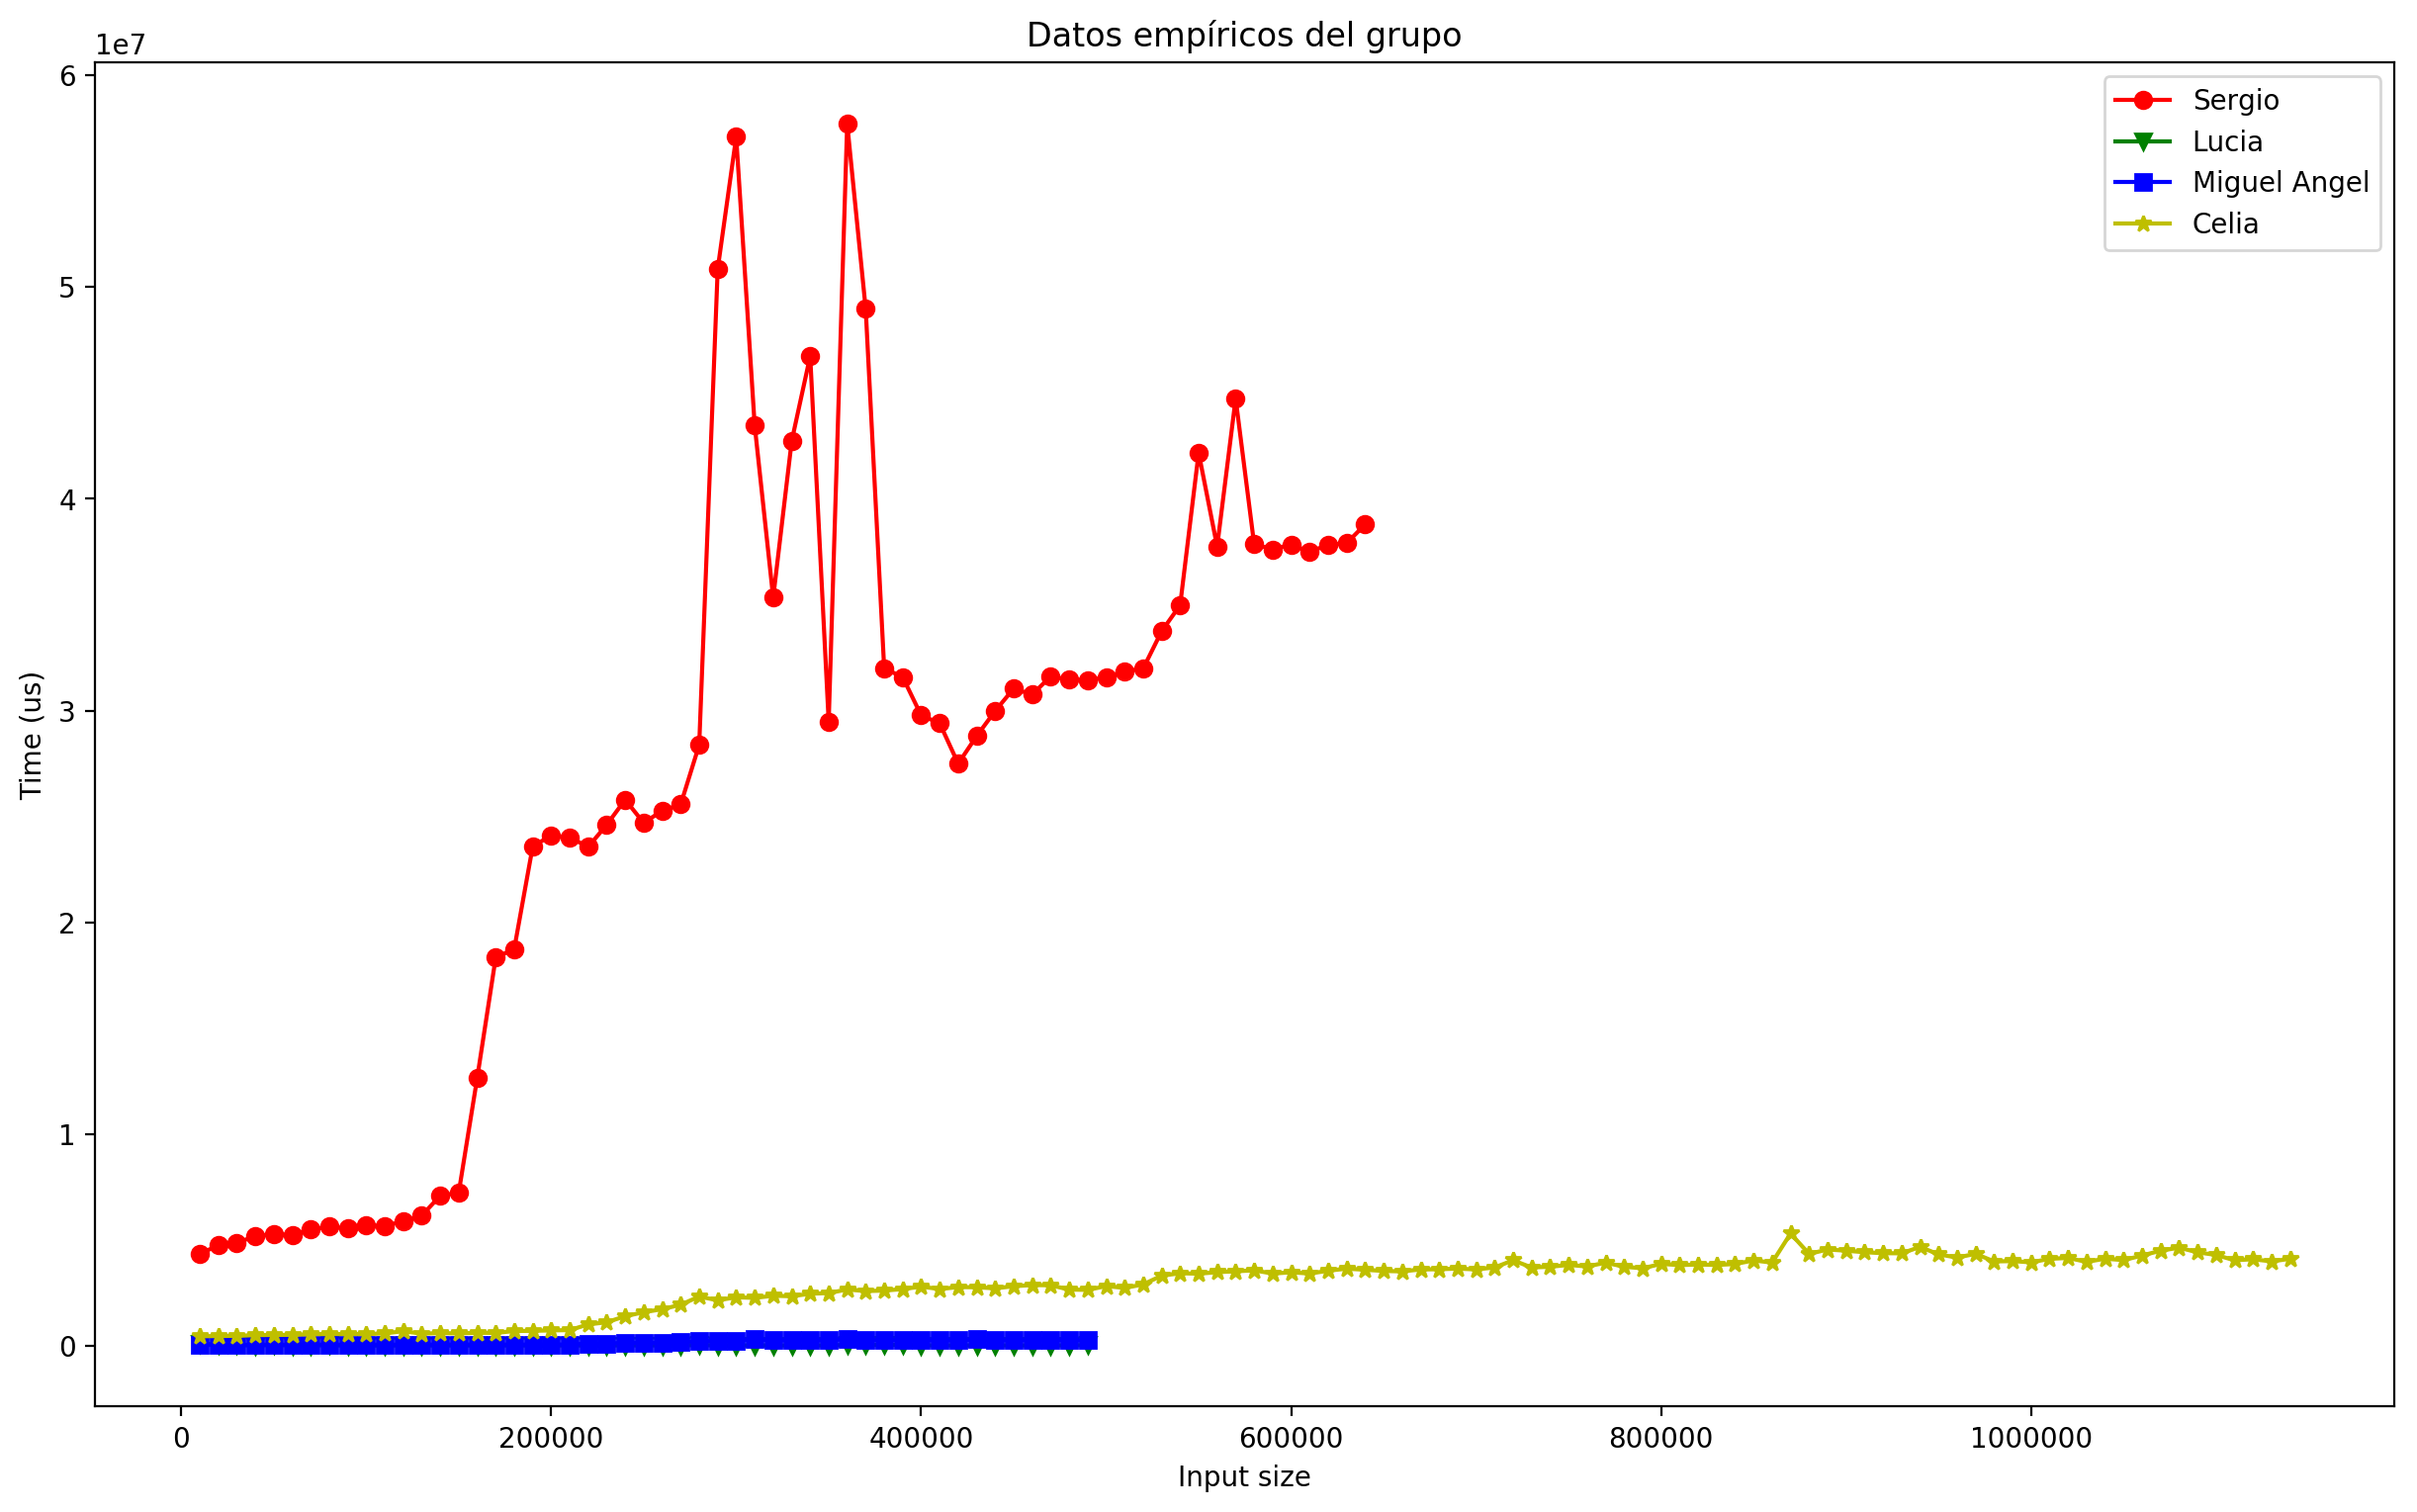
\includegraphics[width=\textwidth]{./Graficas/busquedabinaria_todos.png}
\end{frame}

\begin{frame}[fragile]{Búsqueda binaria (versión recursiva). 
\normalfont{Eficiencia híbrida}}
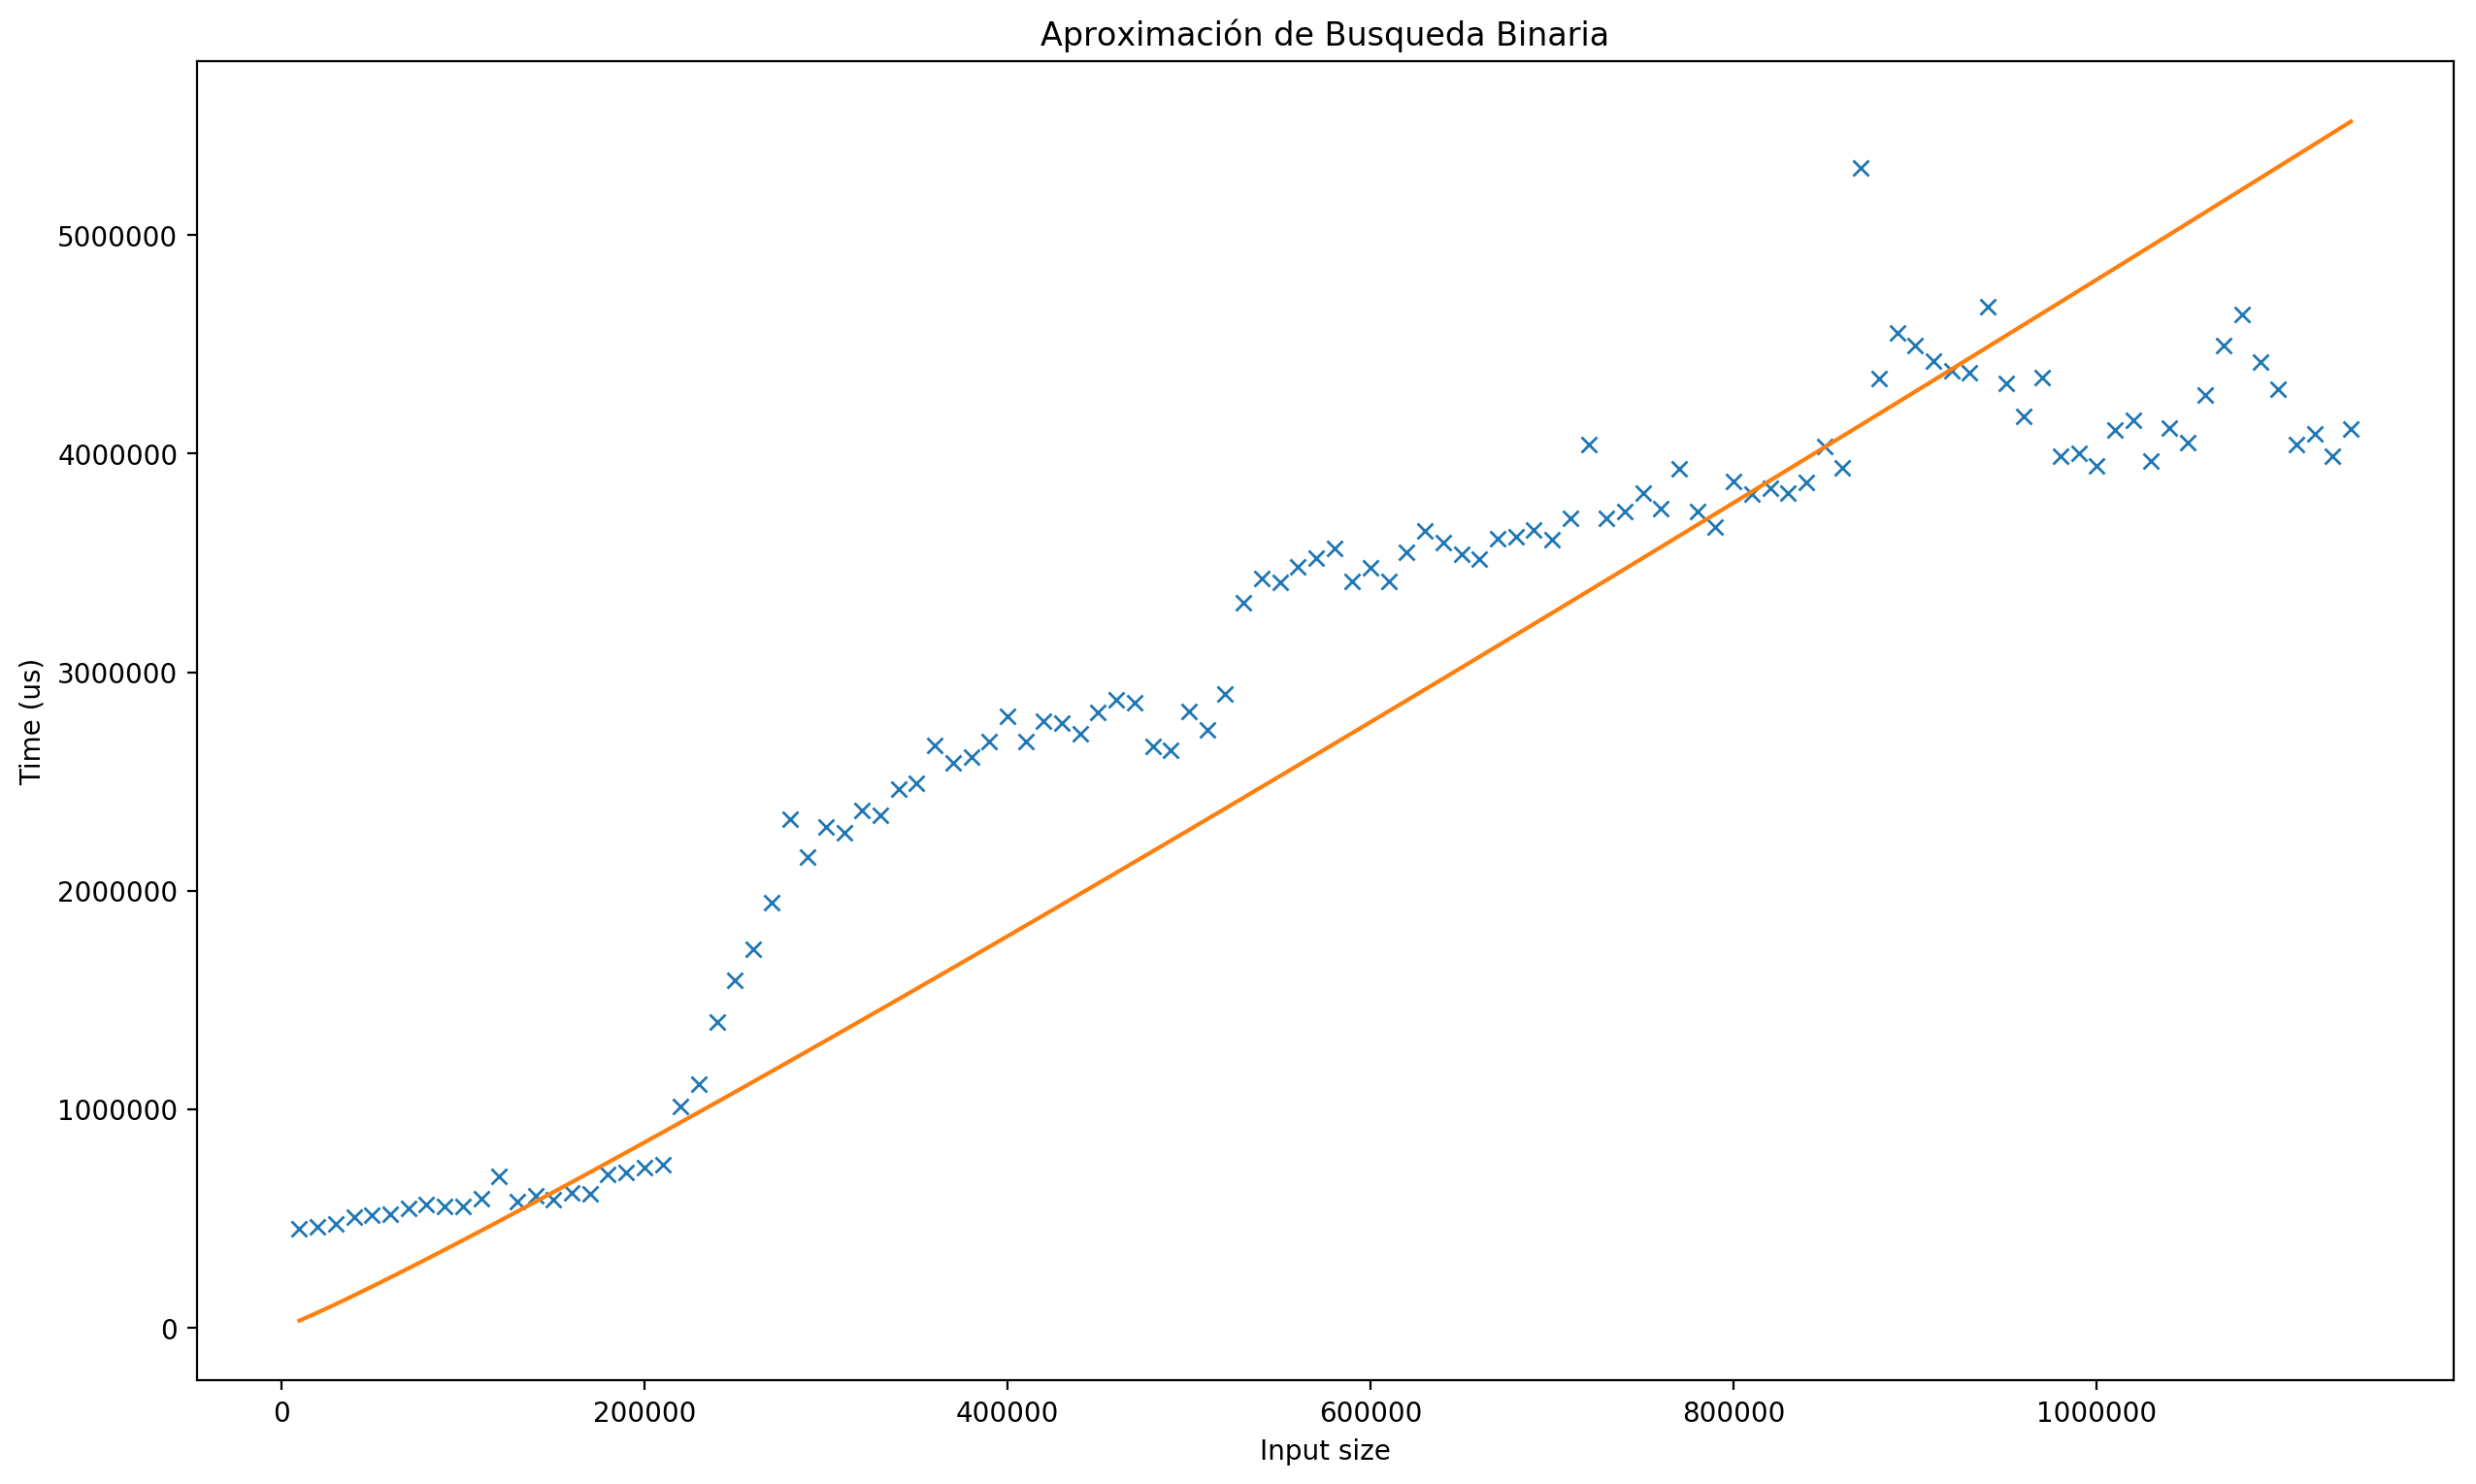
\includegraphics[width=\textwidth]{./Graficas/busquedabinaria_ajuste.png}
\end{frame}

\begin{frame}[fragile]{Búsqueda binaria (versión recursiva). 
	\normalfont{Eficiencia híbrida}}
\textbf{Constante oculta:} $K=0.8630419355569797$

\textbf{Ajuste por regresión:} $T(n)=0.28166261 \cdot n\log n$
\begin{itemize}
	\item \textbf{Error para recta ($kn$): 7.227564149512647\%}
	\item Error para cuadrática ($kn^2$): 56.14209694786215\%
	\item Error para cúbica ($kn^3$): 74.09603399513483\%
	\item Error para logarítmica ($k\log n$): 100.0\%
	\item \textbf{Error para $\boldsymbol{n}$-logarítmica ($\boldsymbol{kn\log n}$): 13.766671701121327\%}
\end{itemize}
\end{frame}

\begin{frame}[fragile]{Heap Sort}
\begin{lstlisting}[language=C]
void heapsort(int T[], int num_elem) {
	for ( int i = num_elem/2; i >= 0; i-- ) {
		reajustar(T, num_elem, i);
	}
	for ( int i = num_elem-1; i >= 1; i-- ) {
		int aux = T[0];
		T[0] = T[i];
		T[i] = aux;
		reajustar(T, i, 0);
	}
}
\end{lstlisting}
\end{frame}

\begin{frame}[fragile]{Heap Sort}
\begin{lstlisting}[language=C]
void reajustar(int T[], int num_elem, int k) {
	int j, v = T[k];
	bool esAPO = false;

	while ( ( k < num_elem/2 ) && !esAPO ) {
		j = 2*k + 1;
		if ( ( j < ( num_elem - 1 ) ) && ( T[j] < T[j+1] ) )
			j++;
		if ( v >= T[j] )
			esAPO = true;
		T[k] = T[j];
		k = j;
	}

	T[k] = v;
}
\end{lstlisting}
\end{frame}

\begin{frame}[fragile]{Heap Sort. 
\normalfont{Eficiencia teórica}}
\begin{center}
	\textbf{\large{Eficiencia de reajustar}}
\end{center}
Queremos el mayor número de iteraciones del bucle ($k \textless \frac{n}{2}$) $$ 0 \leq k \leq n-1$$ No queremos que j incremente $\Rightarrow$ no entra en los \texttt{if}
$$k_i = 2k_{i-1} +c$$ 
Solución de la recurrencia: $$k_i = 2^i -1$$ Siendo el caso inicial $k_0 = 0$

\end{frame}

\begin{frame}[fragile]{Heap Sort. 
\normalfont{Eficiencia teórica}}
\begin{center}
\textbf{\large{Eficiencia de reajustar}}
\end{center}
Queremos que $k = \frac{n}{2}$. Sustituimos $$2^i-1=\frac{n}{2}$$ $$i=\log_2{\frac{n-2}{2}}$$ $$i=\log_2{n-2}-\log_2{2}$$ $$i=\log_2{n-2}-1$$ Tenemos que $$T(n) \in O(\log_2(n))$$

\end{frame}

\begin{frame}[fragile]{Heap Sort. 
\normalfont{Eficiencia teórica}}
\begin{center}
\textbf{\large{Eficiencia de heapsort}}
\end{center}
El primer \texttt{for} hace $\frac{n}{2}$ iteraciones y el segundo \texttt{for} hace $n-1$ iteraciones

Como la eficiencia del interior del \texttt{for} es $O(\log_2{n})$ tenemos que: $$T(n) \in O(n\log_2{n})$$

\end{frame}

\begin{frame}[fragile]{Heap Sort. 
\normalfont{Eficiencia empírica}}
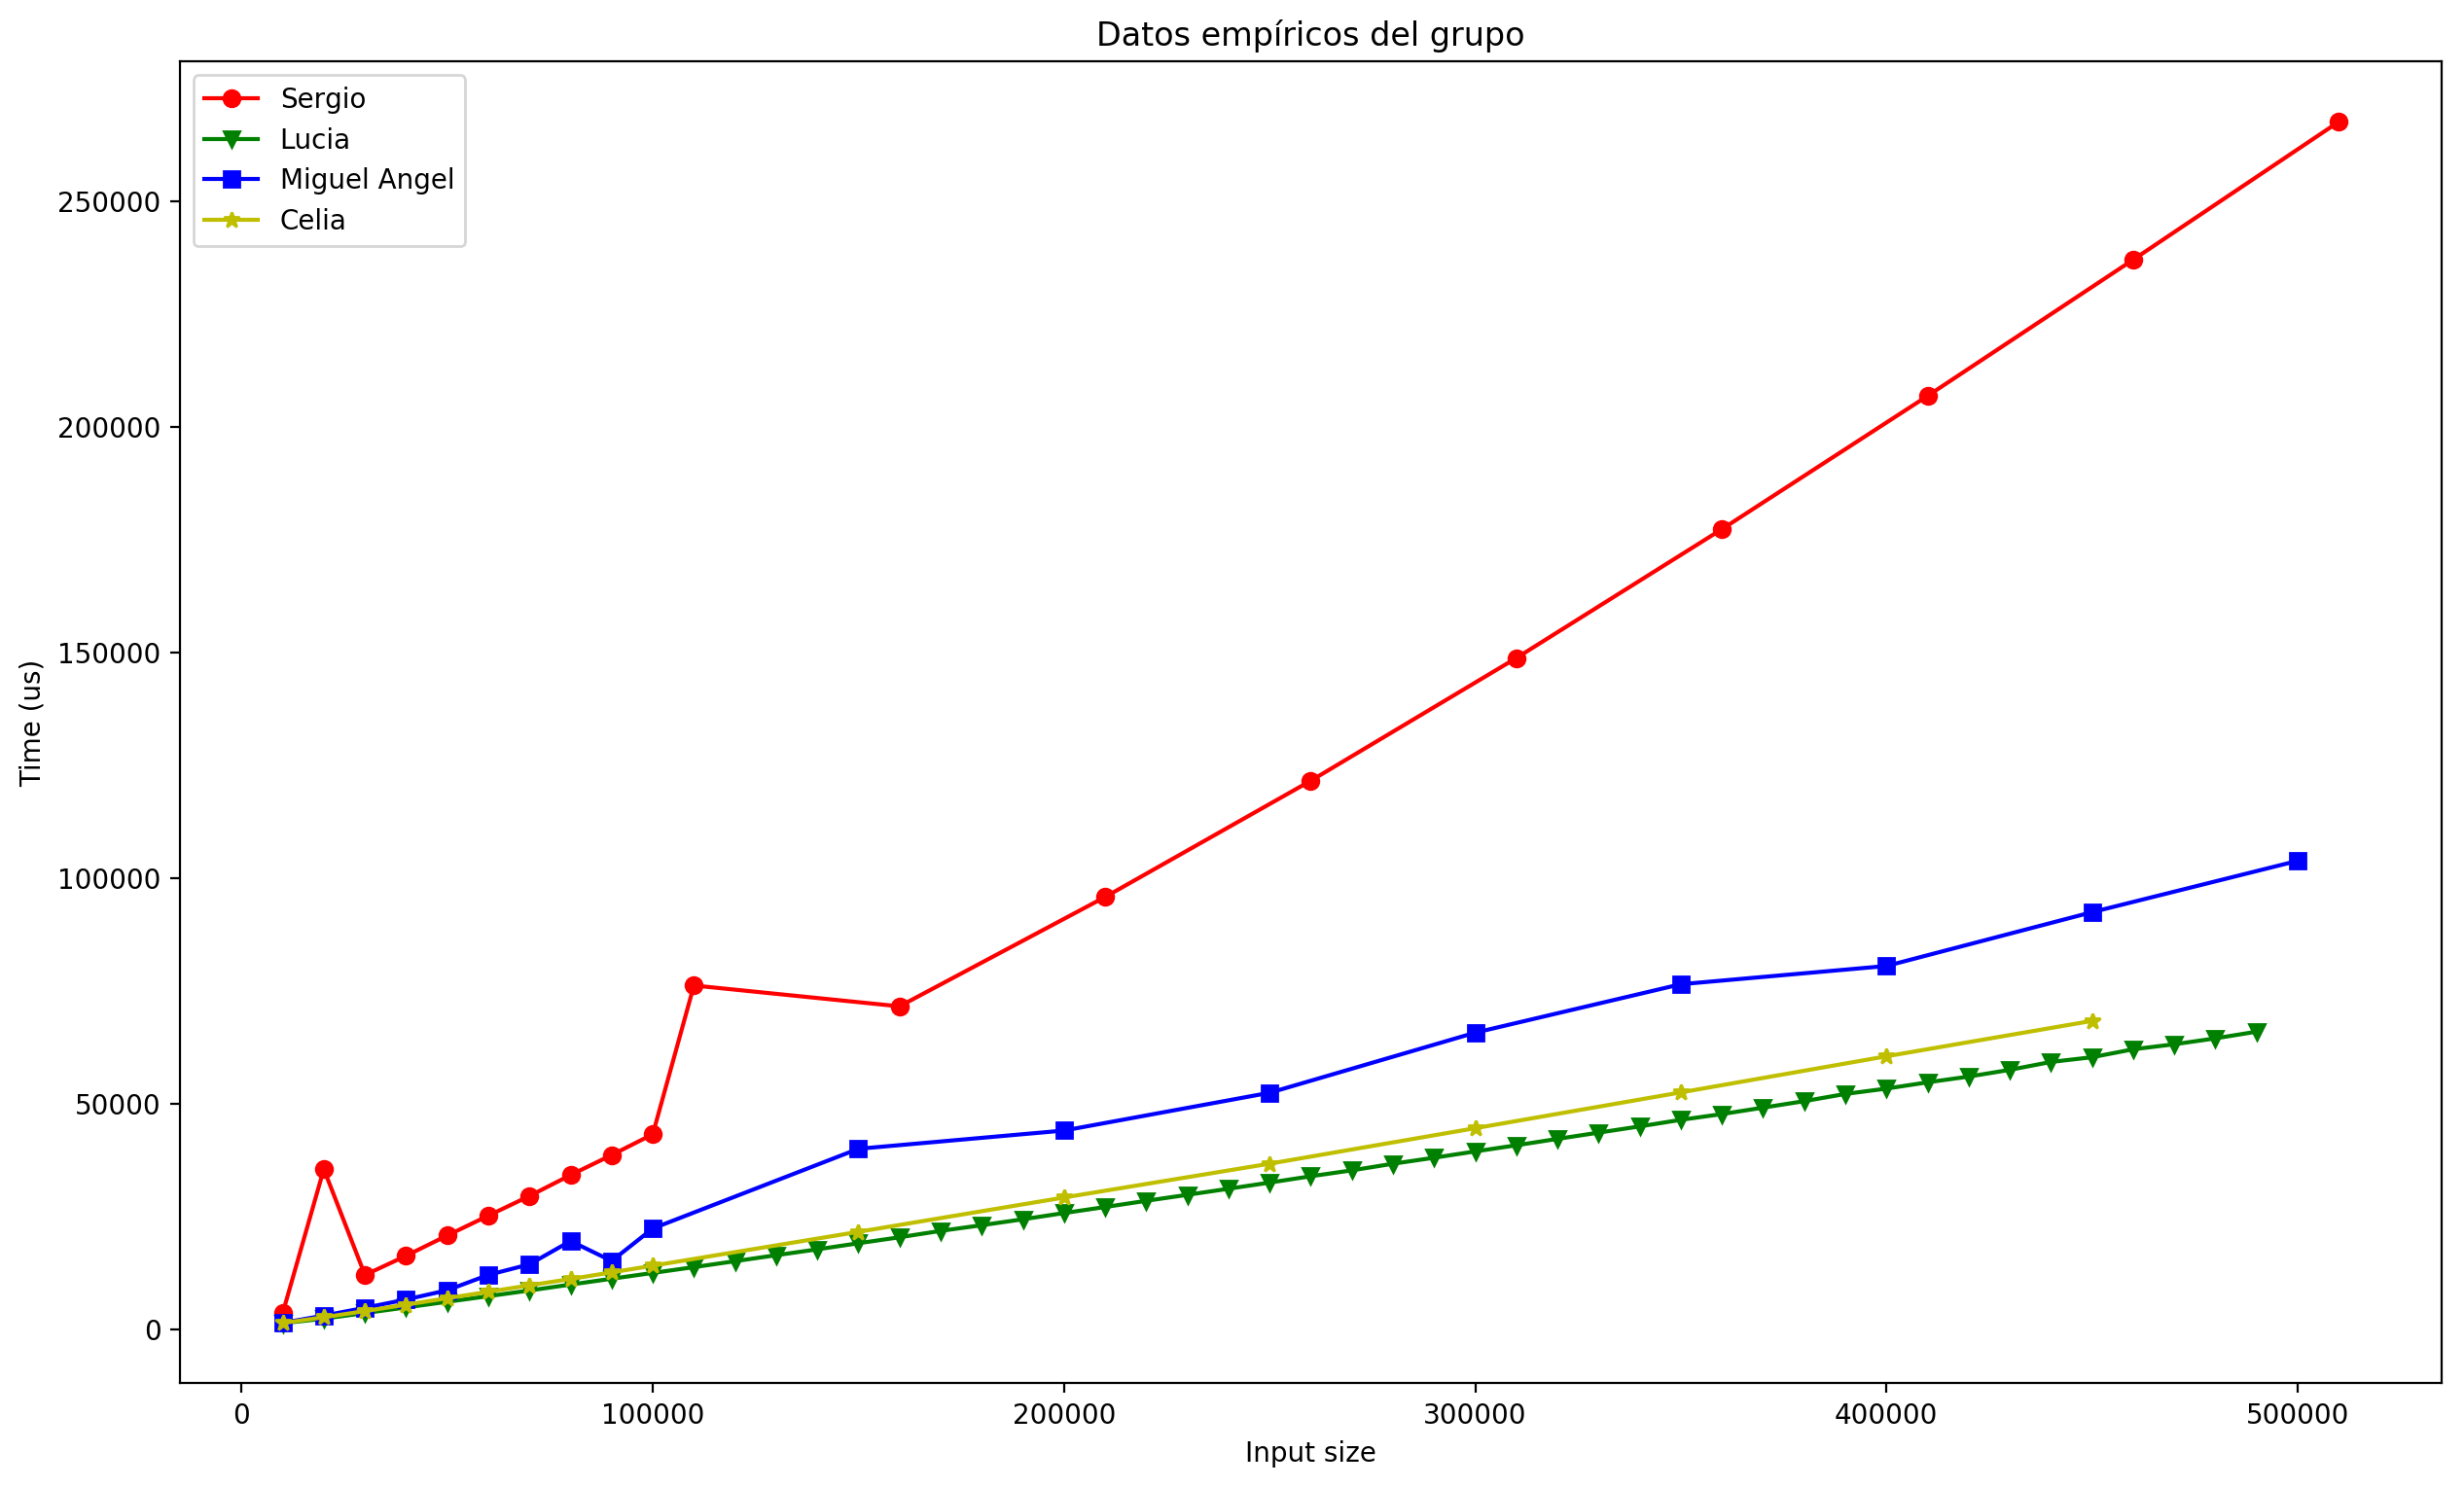
\includegraphics[width=\textwidth]{./Graficas/heap_todos.png}
\end{frame}

\begin{frame}[fragile]{Heap Sort. 
\normalfont{Eficiencia híbrida}}
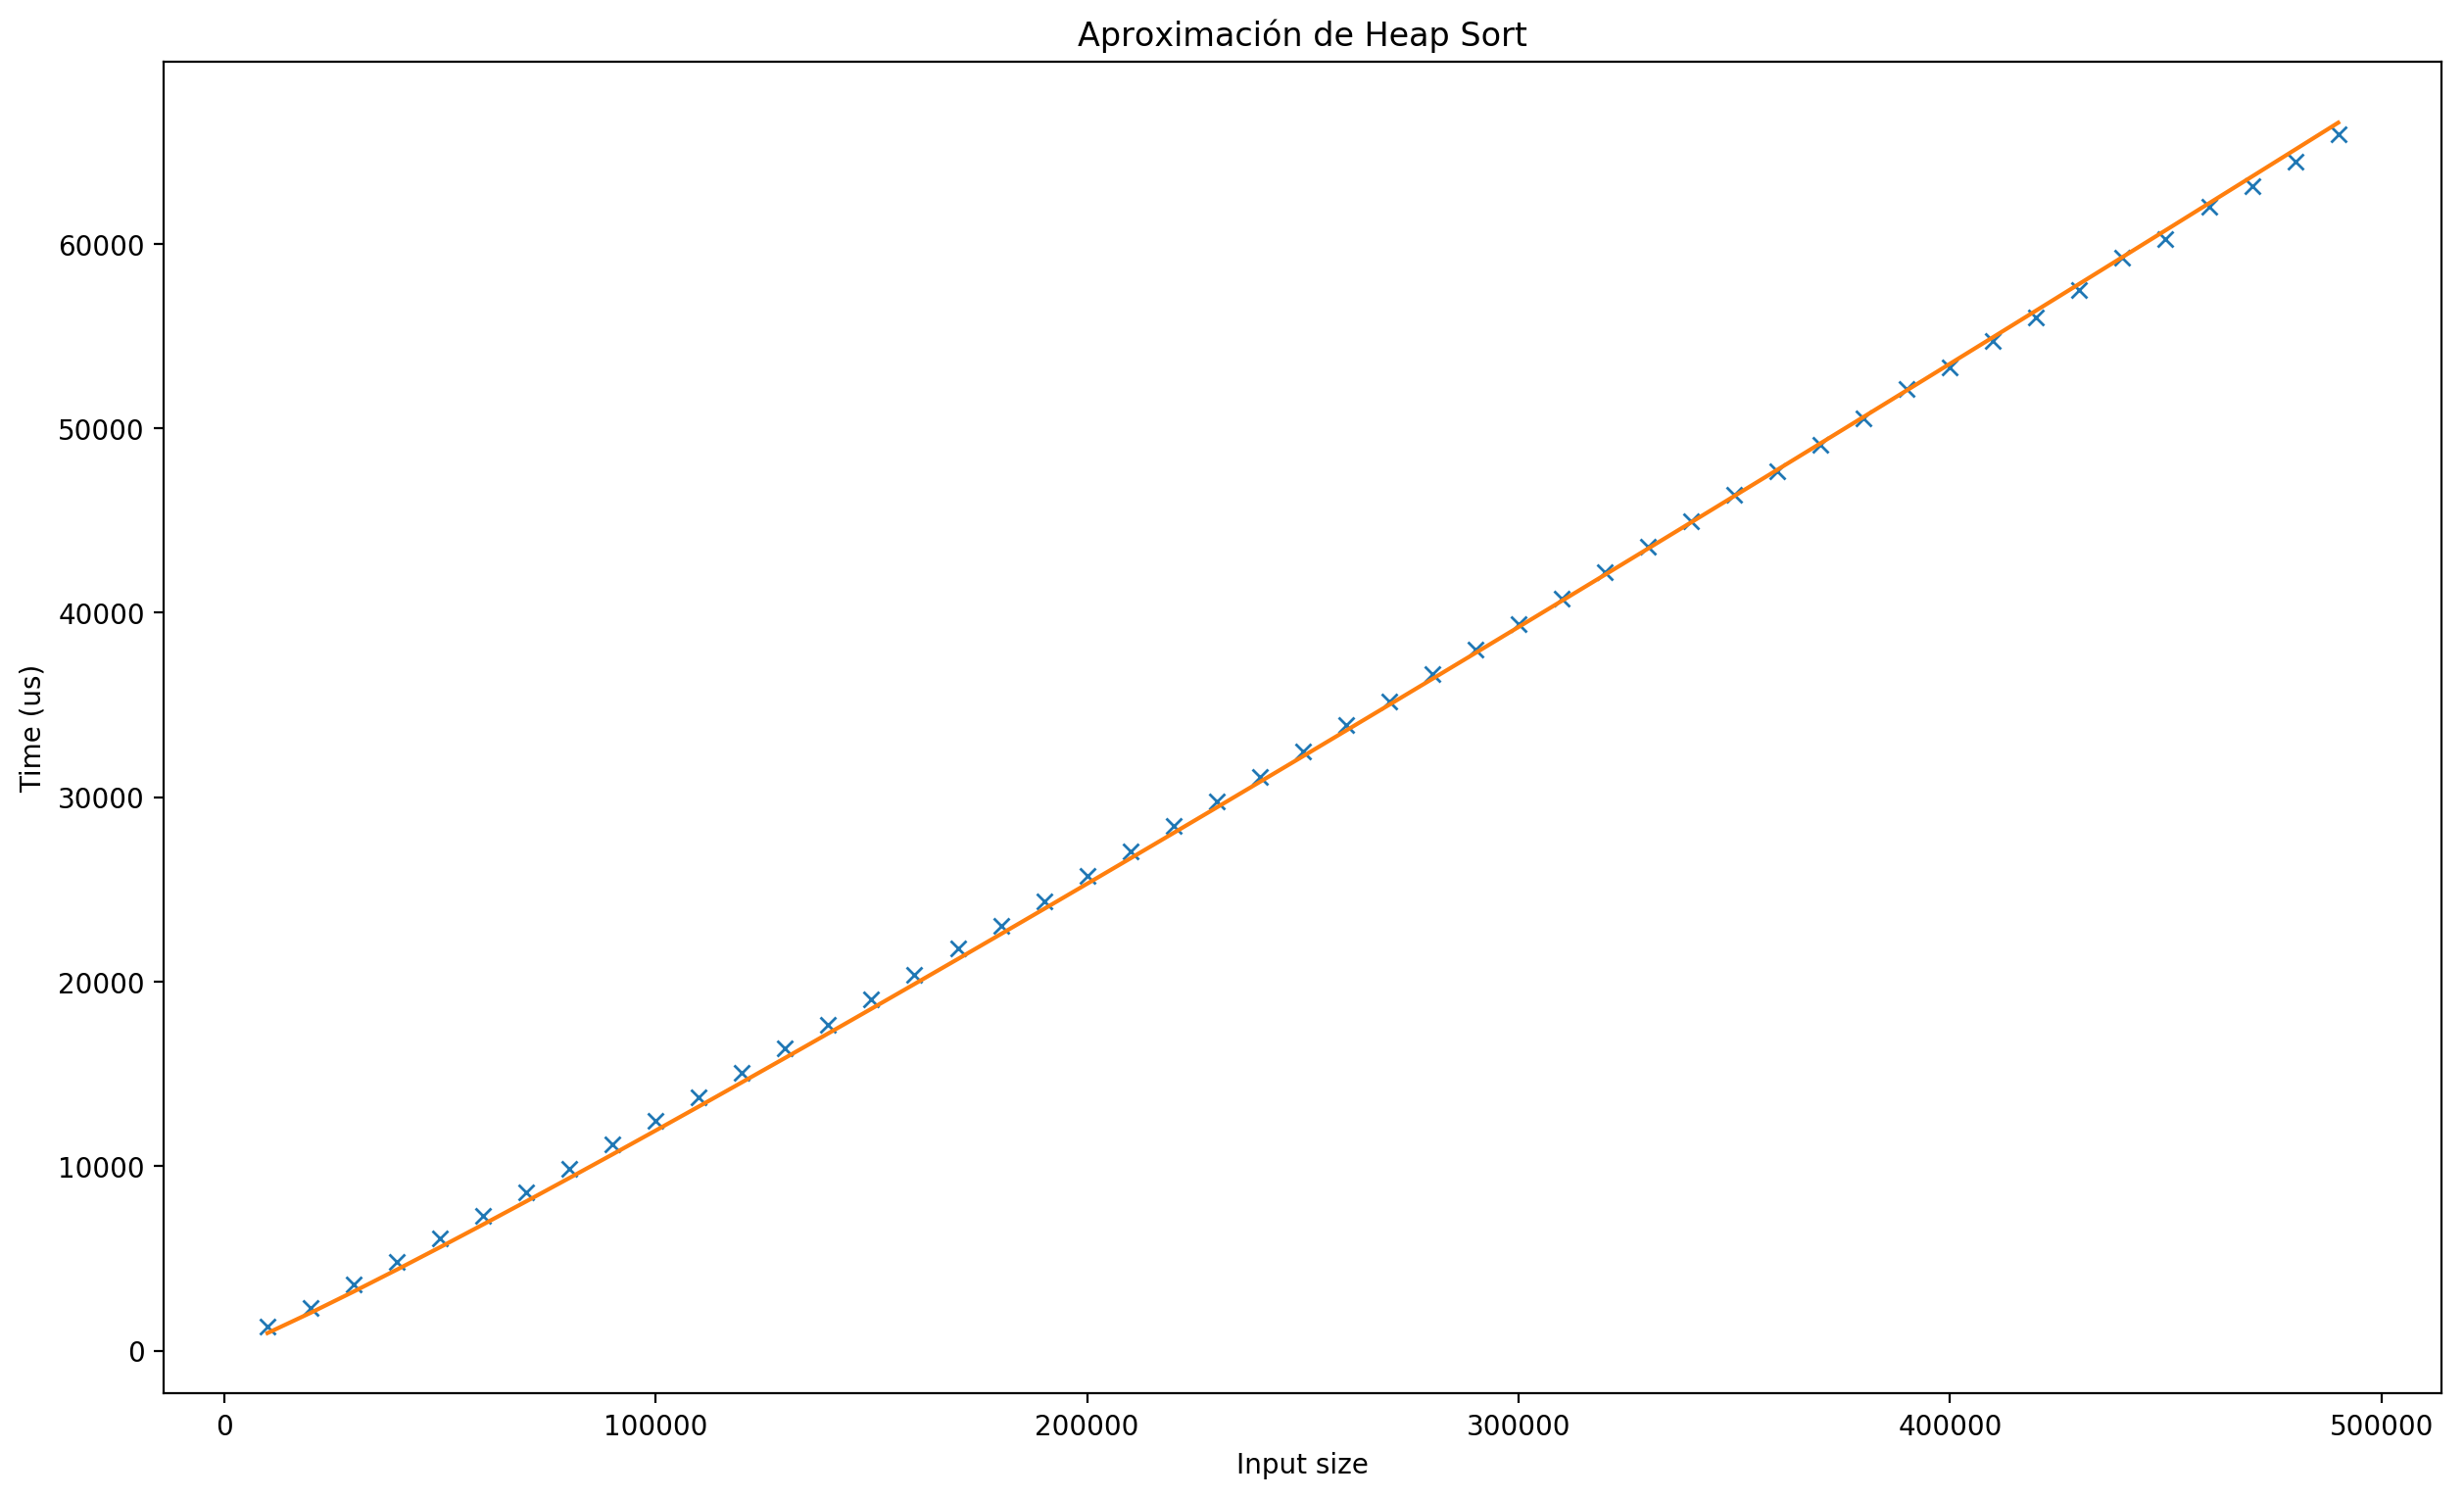
\includegraphics[width=\textwidth]{./Graficas/heap_ajuste.png}
\end{frame}

\begin{frame}[fragile]{Heap Sort. 
	\normalfont{Eficiencia híbrida}}
\textbf{Constante oculta:} $K=0.9753044058661043$

\textbf{Ajuste por regresión:} $T(n)=0.00718669\cdot n \log n$
\begin{itemize}
	\item \textbf{Error para recta ($kn$): 0.04033354197487824\%}
	\item Error para cuadrática ($kn^2$): 27.33530020306984\%
	\item Error para cúbica ($kn^3$): 74.09603399513483\%
	\item Error para logarítmica ($k\log n$): 100.0\%
	\item \textbf{Error para $\boldsymbol{n}$-logarítmica ($\boldsymbol{kn\log n}$): 0.04894682223025979\%}
\end{itemize}
\end{frame}

\begin{frame}[fragile]{Bubble Sort}
\begin{lstlisting}[language=C]
void burbuja(int v[], int n) {
	int aux;

	for ( int i = inicial, i < final-1; i++ ) {
		for ( j = final-1; j > i; j-- ) {
			if ( v[j] < v[j-1] ) {
				aux = v[j];
				v[j] = v[j-1];
				v[j-1] = aux;
			}
		}
	}
}
\end{lstlisting}
\end{frame}

\begin{frame}[fragile]{Bubble Sort. 
\normalfont{Eficiencia teórica}}
El \texttt{for} interno se ejecuta desde \texttt{fin-1} hasta \texttt{i} iteraciones y se ejecuta desde 0 hasta \texttt{fin-2}. $$T(n)=\sum_{i=0}^{n-1}{n-i-1}=n^2-\frac{(n-2)(n-1)}{2}-5$$
Por lo tanto $$T(n) \in O(n^2)$$


\end{frame}

\begin{frame}[fragile]{Bubble Sort. 
\normalfont{Eficiencia empírica}}
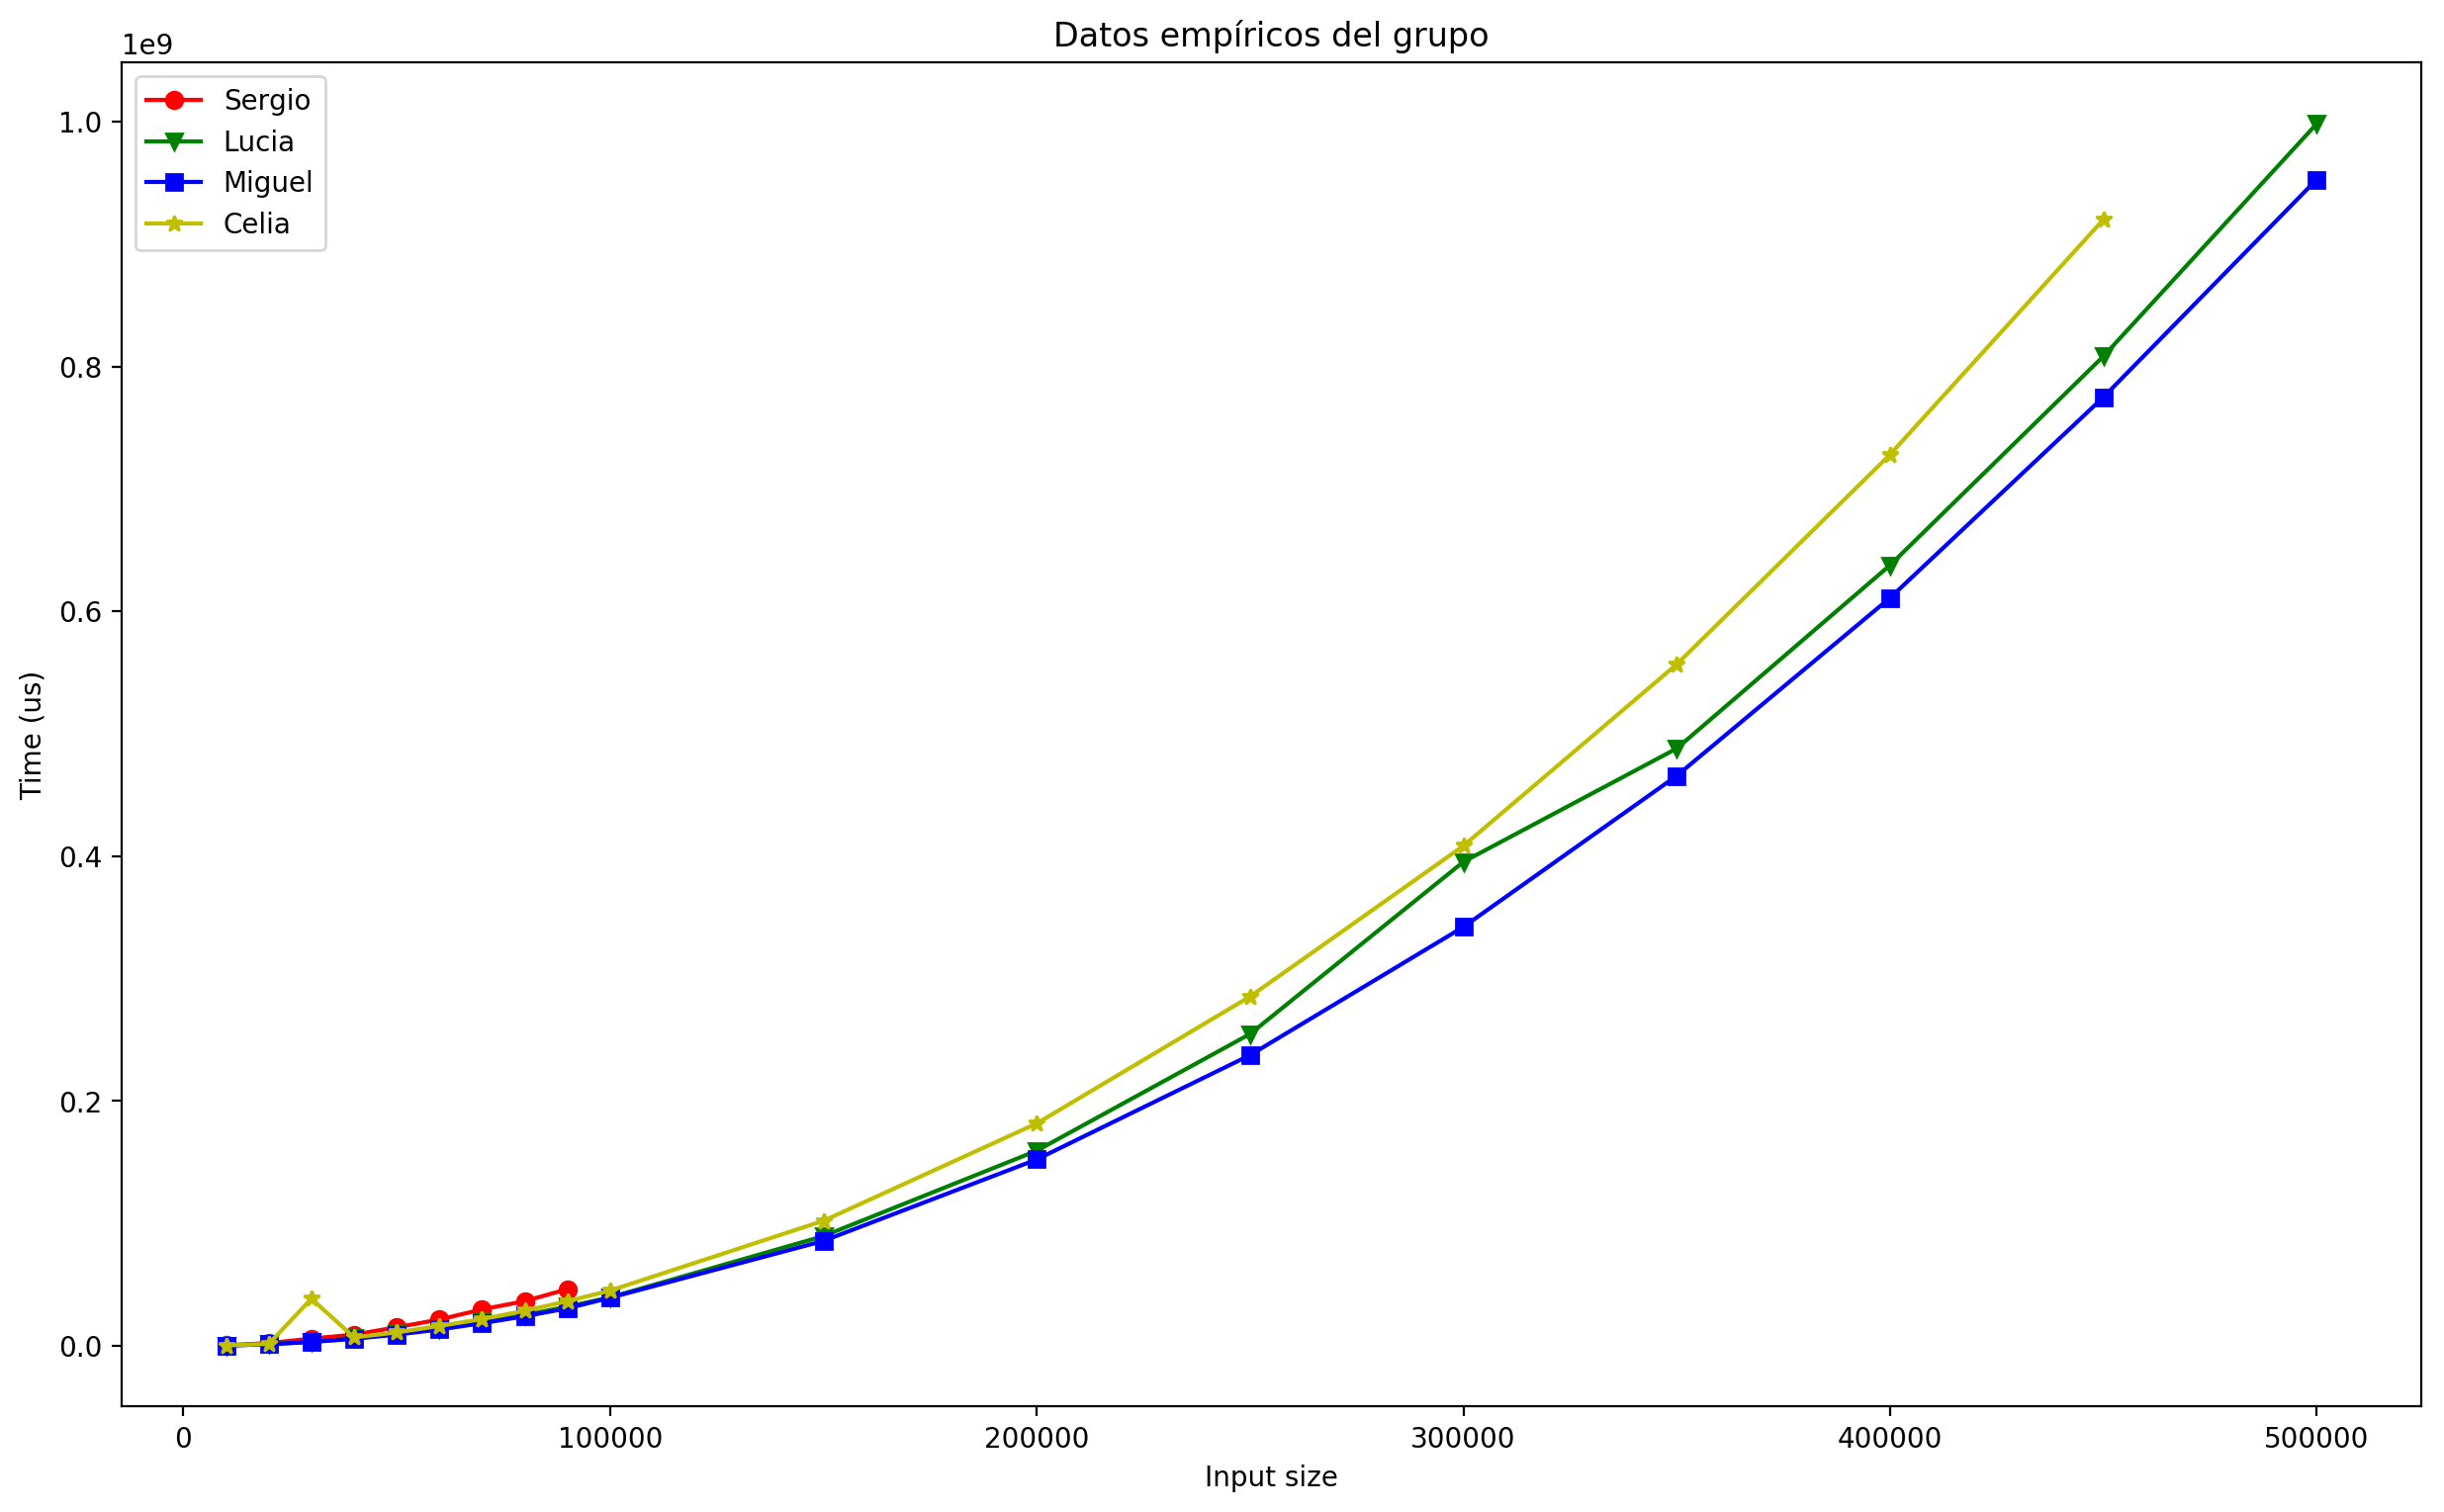
\includegraphics[width=\textwidth]{./Graficas/bubble_todos.png}
\end{frame}

\begin{frame}[fragile]{Bubble Sort. 
\normalfont{Eficiencia híbrida}}
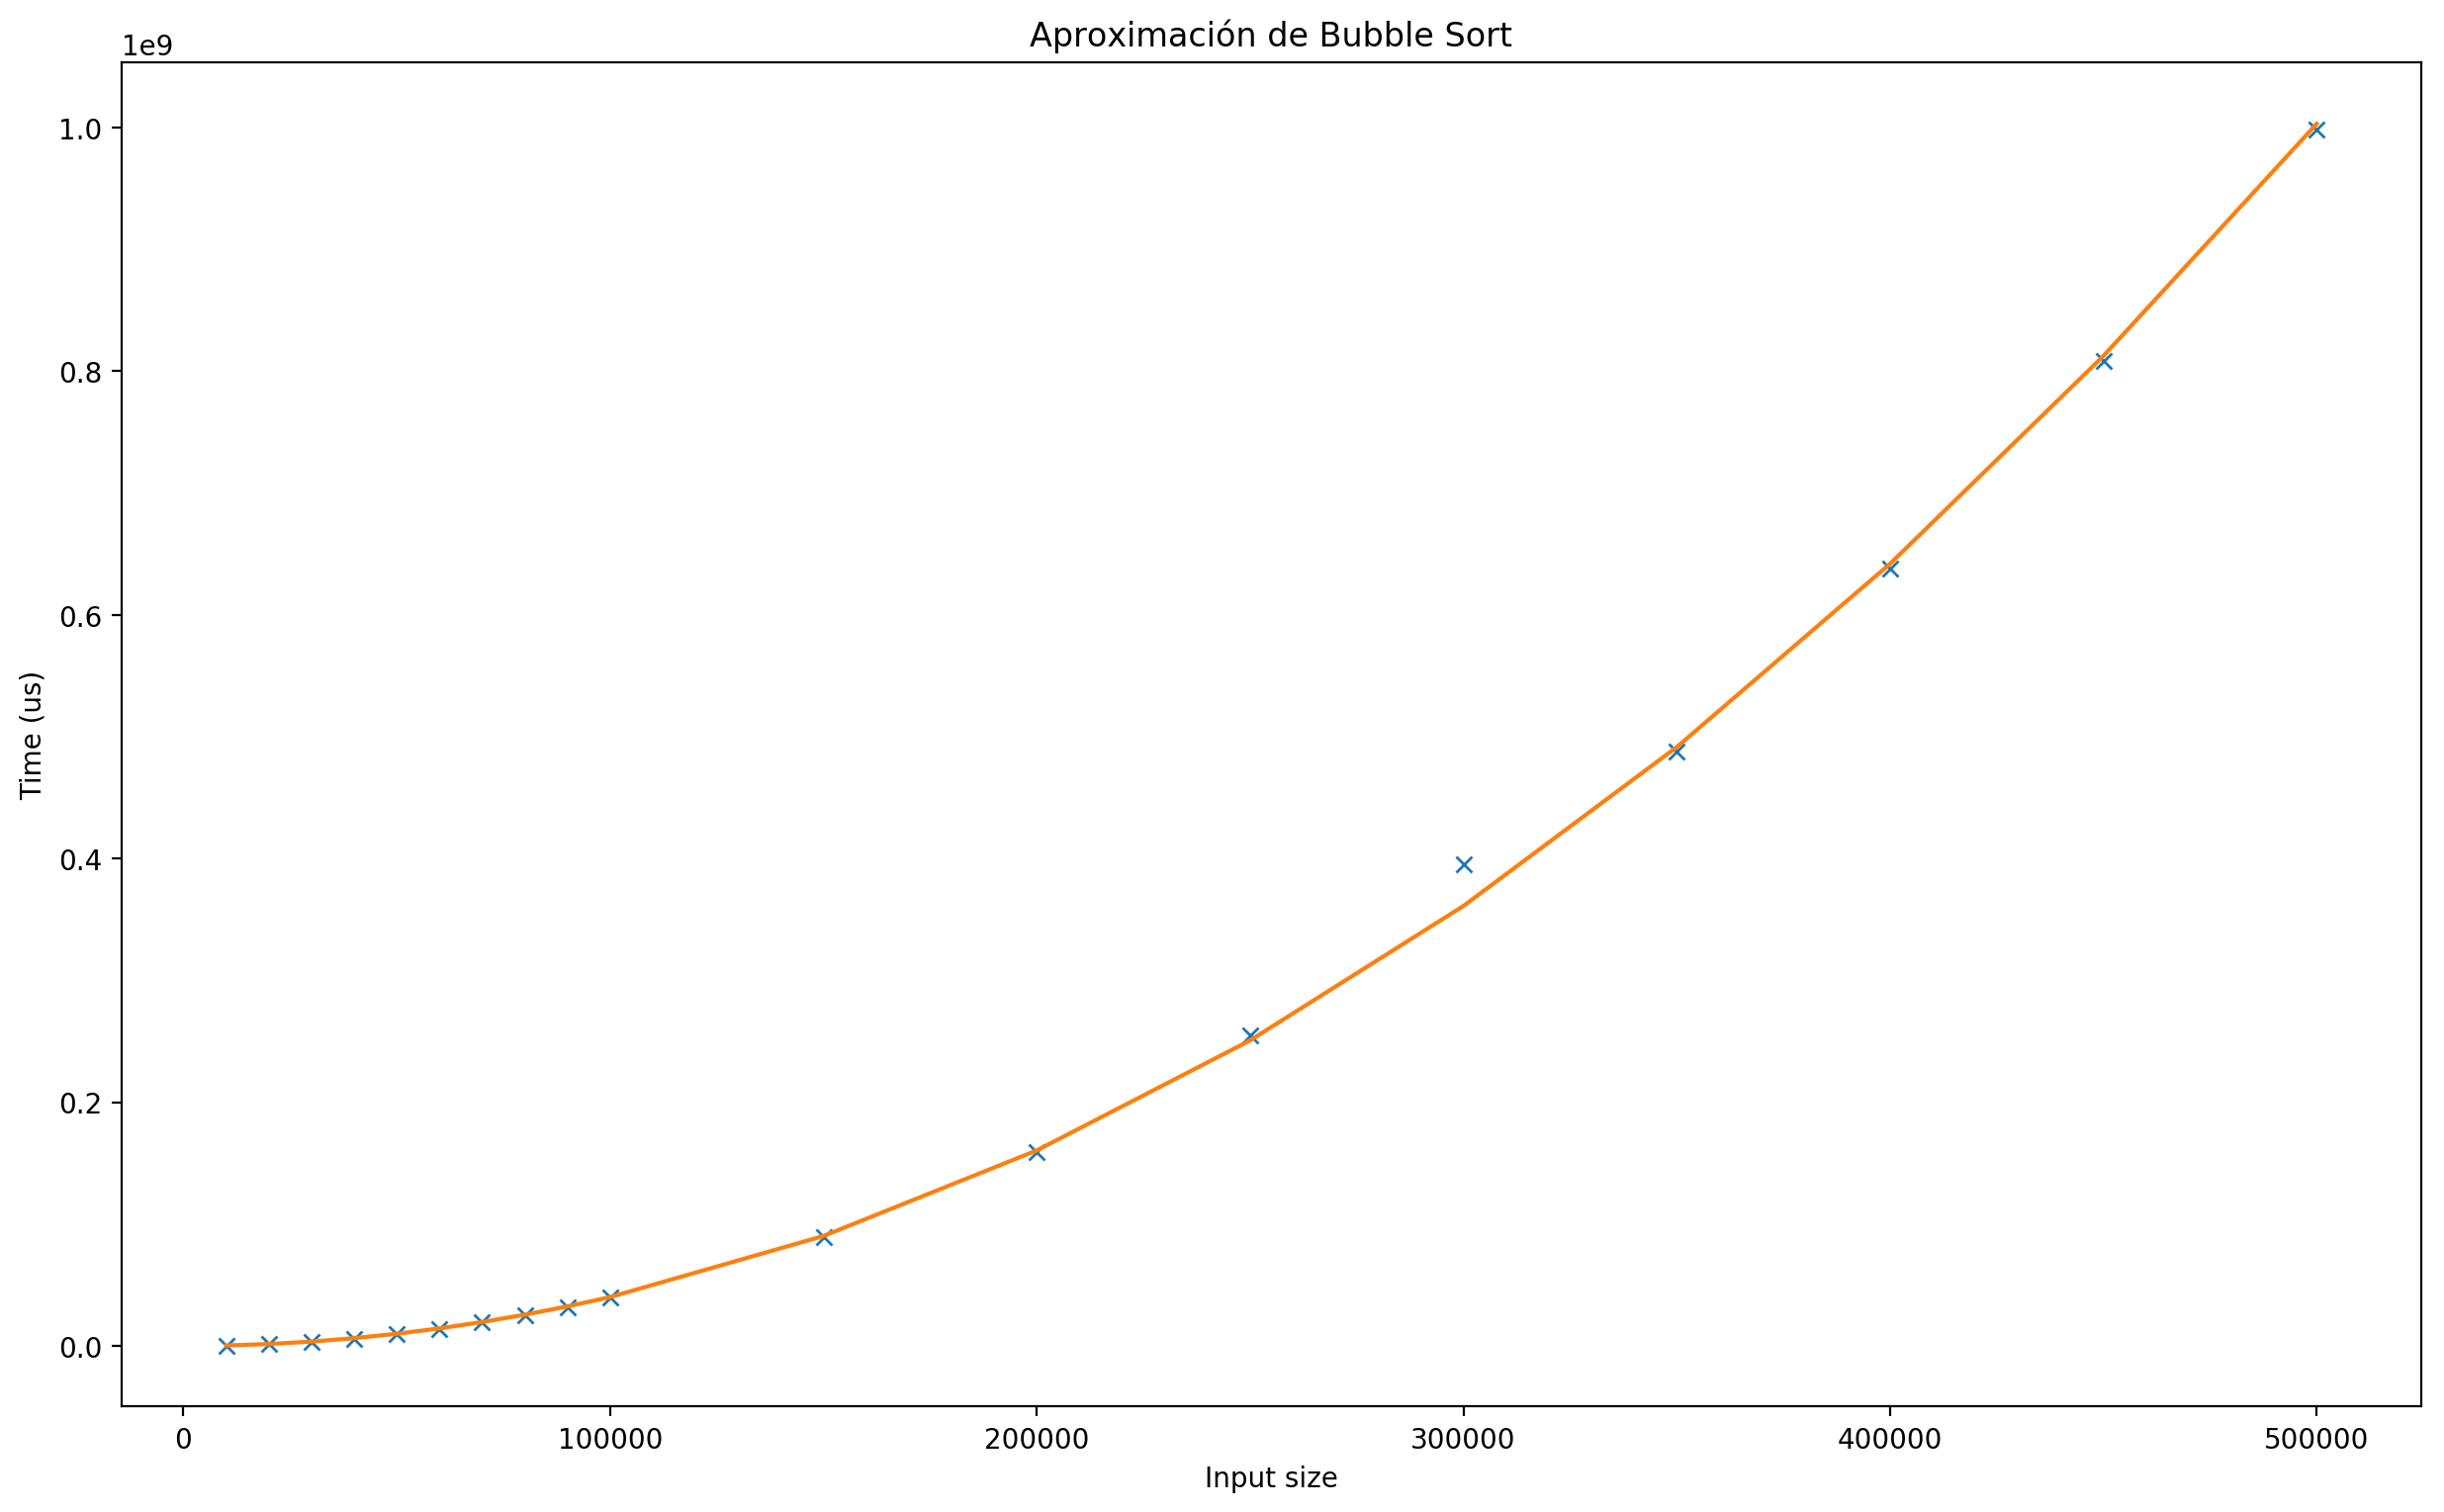
\includegraphics[width=\textwidth]{./Graficas/bubble_ajuste.png}
\end{frame}

\begin{frame}[fragile]{Bubble Sort. 
	\normalfont{Eficiencia híbrida}}
\textbf{Constante oculta:} $K=1.019659179330859$

\textbf{Ajuste por regresión:} $T(n)=0.00401246\cdot n^2$
\begin{itemize}
	\item Error para recta ($kn$): 6.15853318137504\%
	\item \textbf{Error para cuadrática ($kn^2$): 0.08527050249560174\%}
	\item Error para cúbica ($kn^3$): 5.41027219494451\%
	\item Error para logarítmica ($k\log n$): 100.0\%
	\item Error para $n$-logarítmica ($kn\log n$): 10.096552530276018\%
\end{itemize}
\end{frame}

\begin{frame}[fragile]{Merge Sort}
\begin{lstlisting}[language=C]
static void mergesort_lims(int T[], int inicial, int final) {
	if ( final-inicial < UMBRAL_MS ) 
		insercion_lims(T, inicial, final);
	else {
		int k = (final - inicial)/2;
		int * U = new int [k - inicial + 1];
		assert(U); int l, l2;
		for (l = 0, l2 = inicial; l < k; l++, l2++)
			U[l] = T[l2];
		U[l] = INT_MAX;
		int * V = new int [final - k + 1];
		assert(V);
		for (l = 0, l2 = k; l < final - k; l++, l2++) 
			V[l] = T[l2];
		V[l] = INT_MAX;
		mergesort_lims(U, 0, k); mergesort_lims(V, 0, final-k);
		fusion(T, inicial, final, U, V);
		delete[] U; delete[] V;
	}
}
\end{lstlisting}
\end{frame}

\begin{frame}[fragile]{Merge Sort}
\begin{lstlisting}[language=C]
static void fusion(int T[], int inicial, int final, int U[], int V[]) {
	int j = 0, k = 0;
	for ( int i = inicial; i < final; i++ ) {
		if (U[j] < V[k]) {
			T[i] = U[j];
			j++;
		} else {
			T[i] = V[k];
			k++;
		}
	}
}
\end{lstlisting}
\end{frame}
\begin{frame}[fragile]{Merge Sort. 
\normalfont{Eficiencia teórica}}
\begin{center}
\textbf{\large{Eficiencia de fusión}}
\end{center}
Tiene un bucle \texttt{for} que se repite \texttt{final-inicial} por tanto:$$T(n) \in O(n)$$
\end{frame}

\begin{frame}[fragile]{Merge Sort. 
\normalfont{Eficiencia teórica}}
\begin{center}
\textbf{\large{Eficiencia de mergesort}}
\end{center}
Las dos llamadas a mergesort se hacen sobre vectores cuyo tamaño es la mitad que el original. $$T(m) = 2T\left(\frac{m}{2}\right)+n$$ Sustituyendo m por $2^k$ y despejando: $$T(2^k)-2T(2^{k-1}) = 2^k$$ $$(x-2)^2 = 0$$ $$T(k) = c_1*2^k + c_2*k*2^k$$ $$T(n)=c_1*n+c_2*\log_2{n}*n$$ Obtenemos que: $$T(n) \in O(n\log_2{n})$$

\small{\textit{Observación}: para tamaños pequeños se ejecutará inserción ($O(n^2)$) }

\end{frame}

\begin{frame}[fragile]{Merge Sort. 
\normalfont{Eficiencia empírica}}
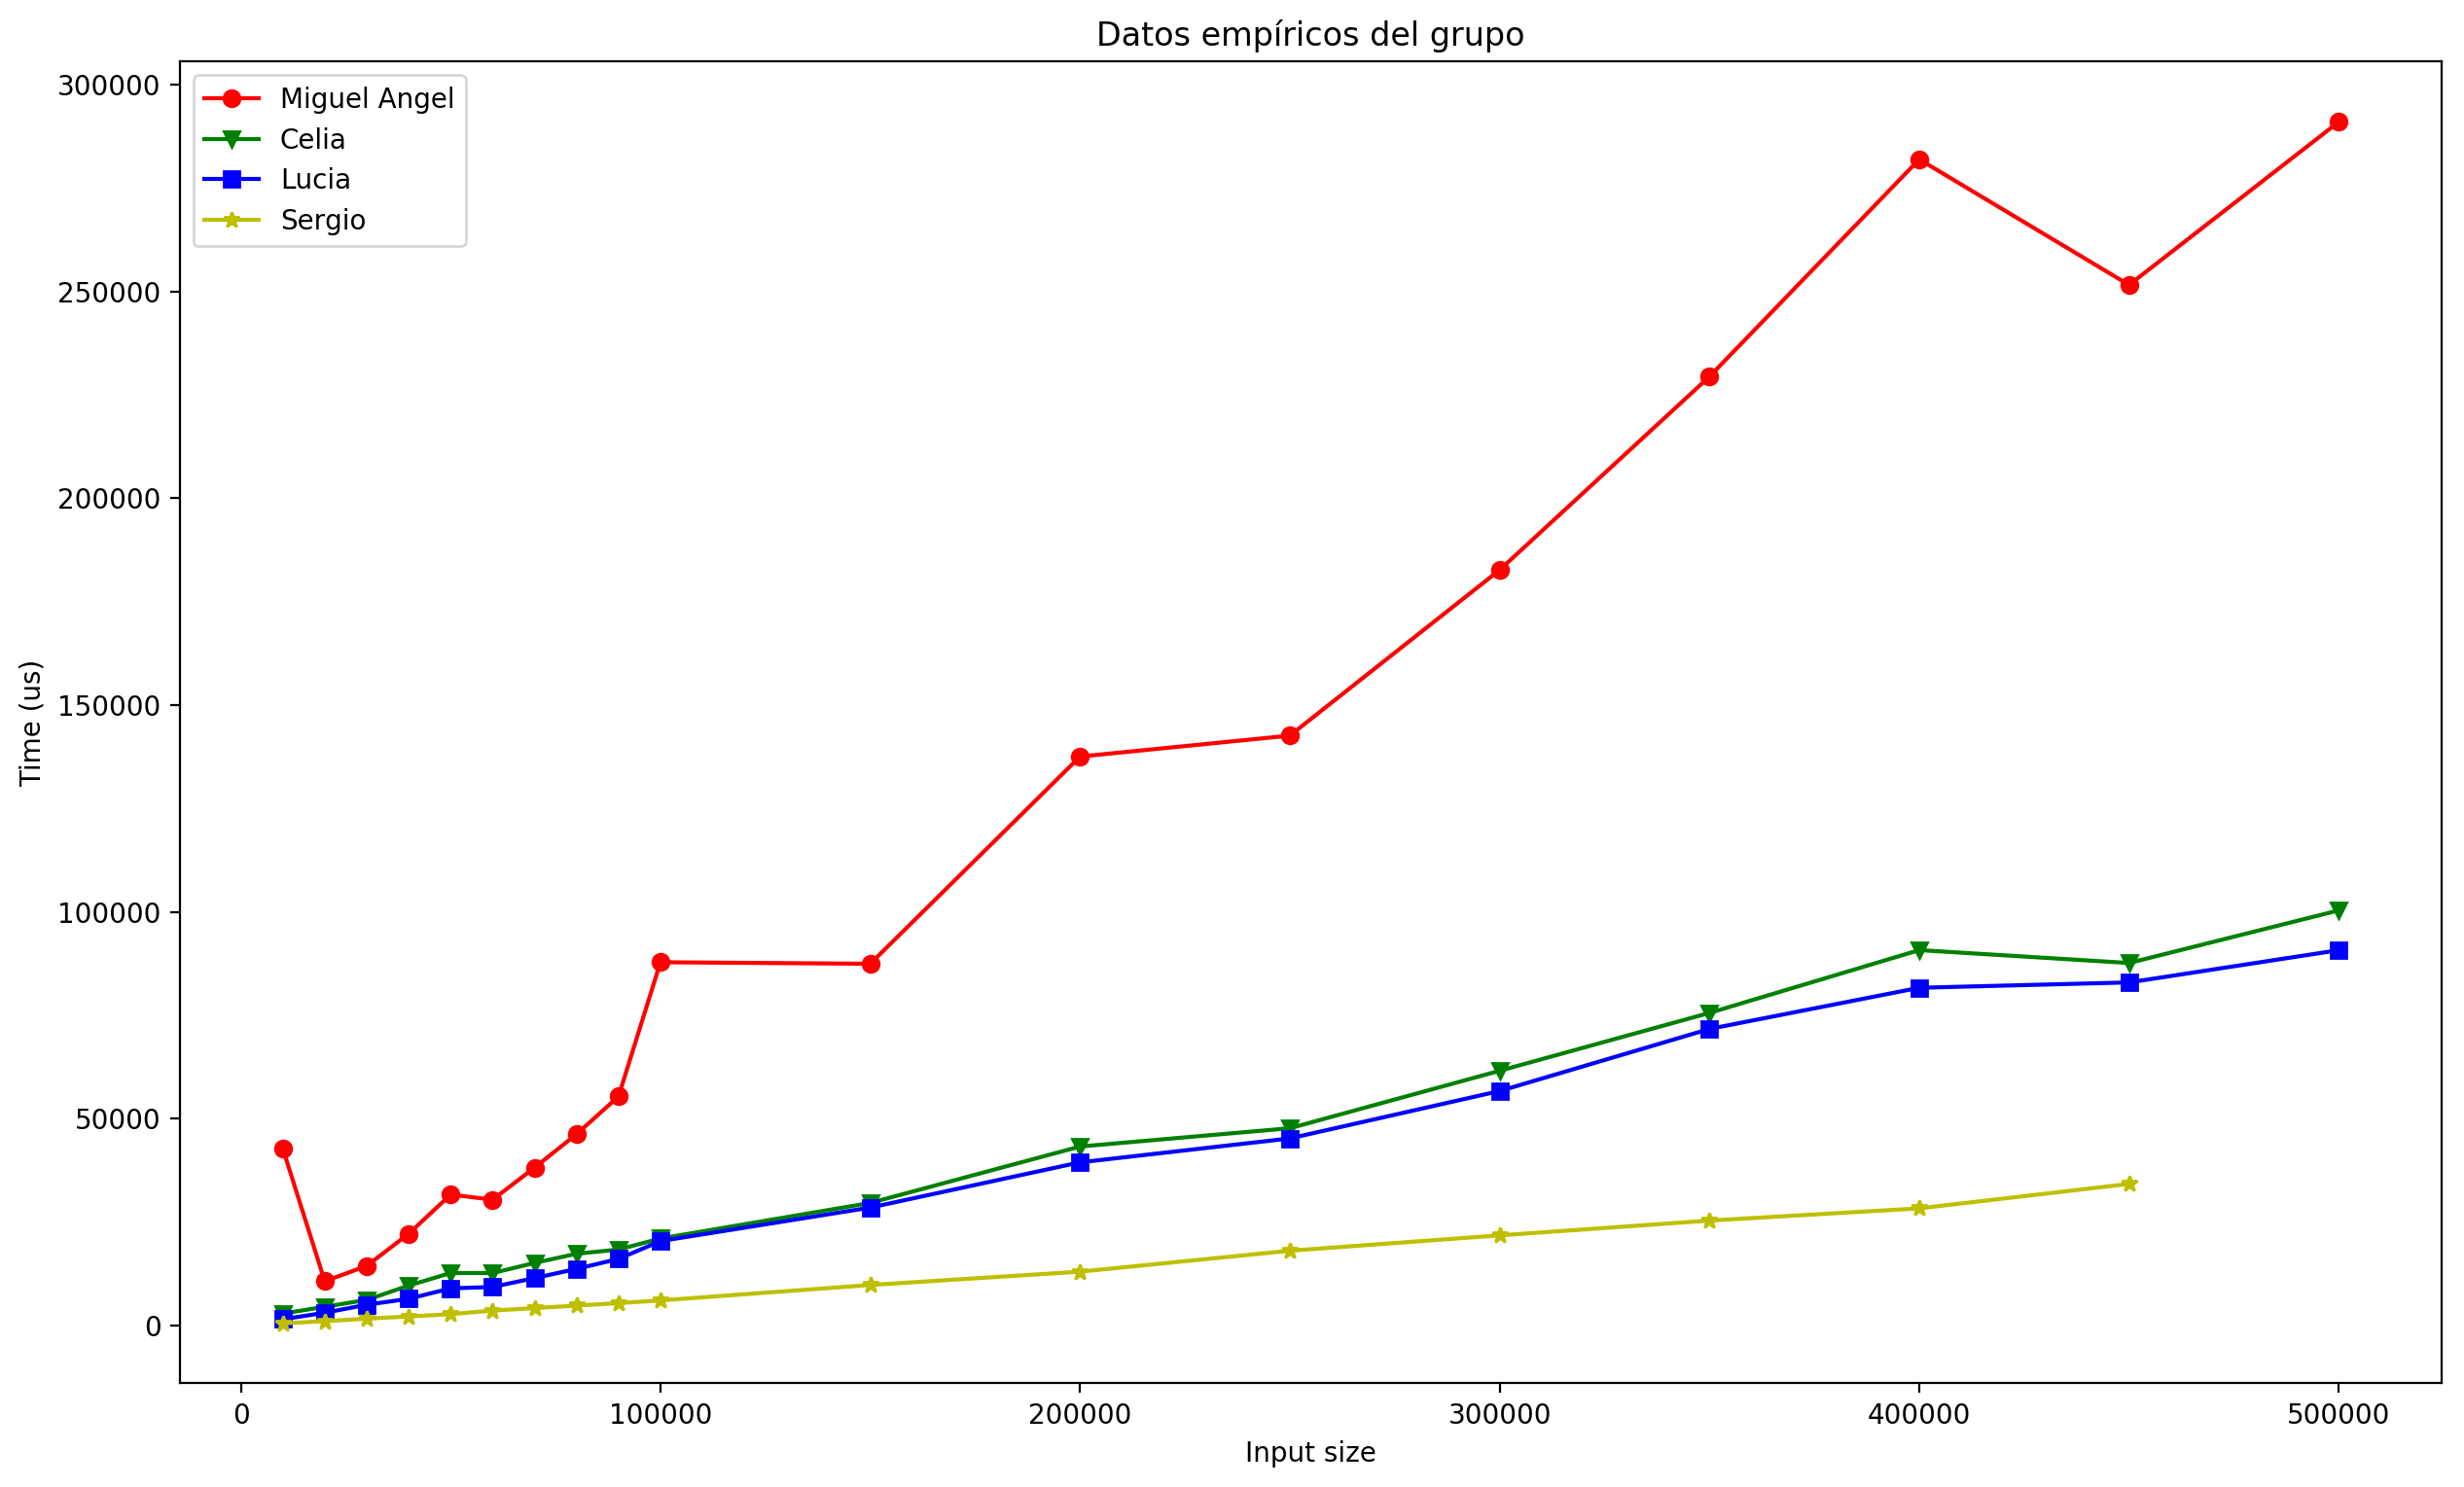
\includegraphics[width=\textwidth]{./Graficas/merge_todos.png}
\end{frame}

\begin{frame}[fragile]{Merge Sort. 
\normalfont{Eficiencia híbrida}}
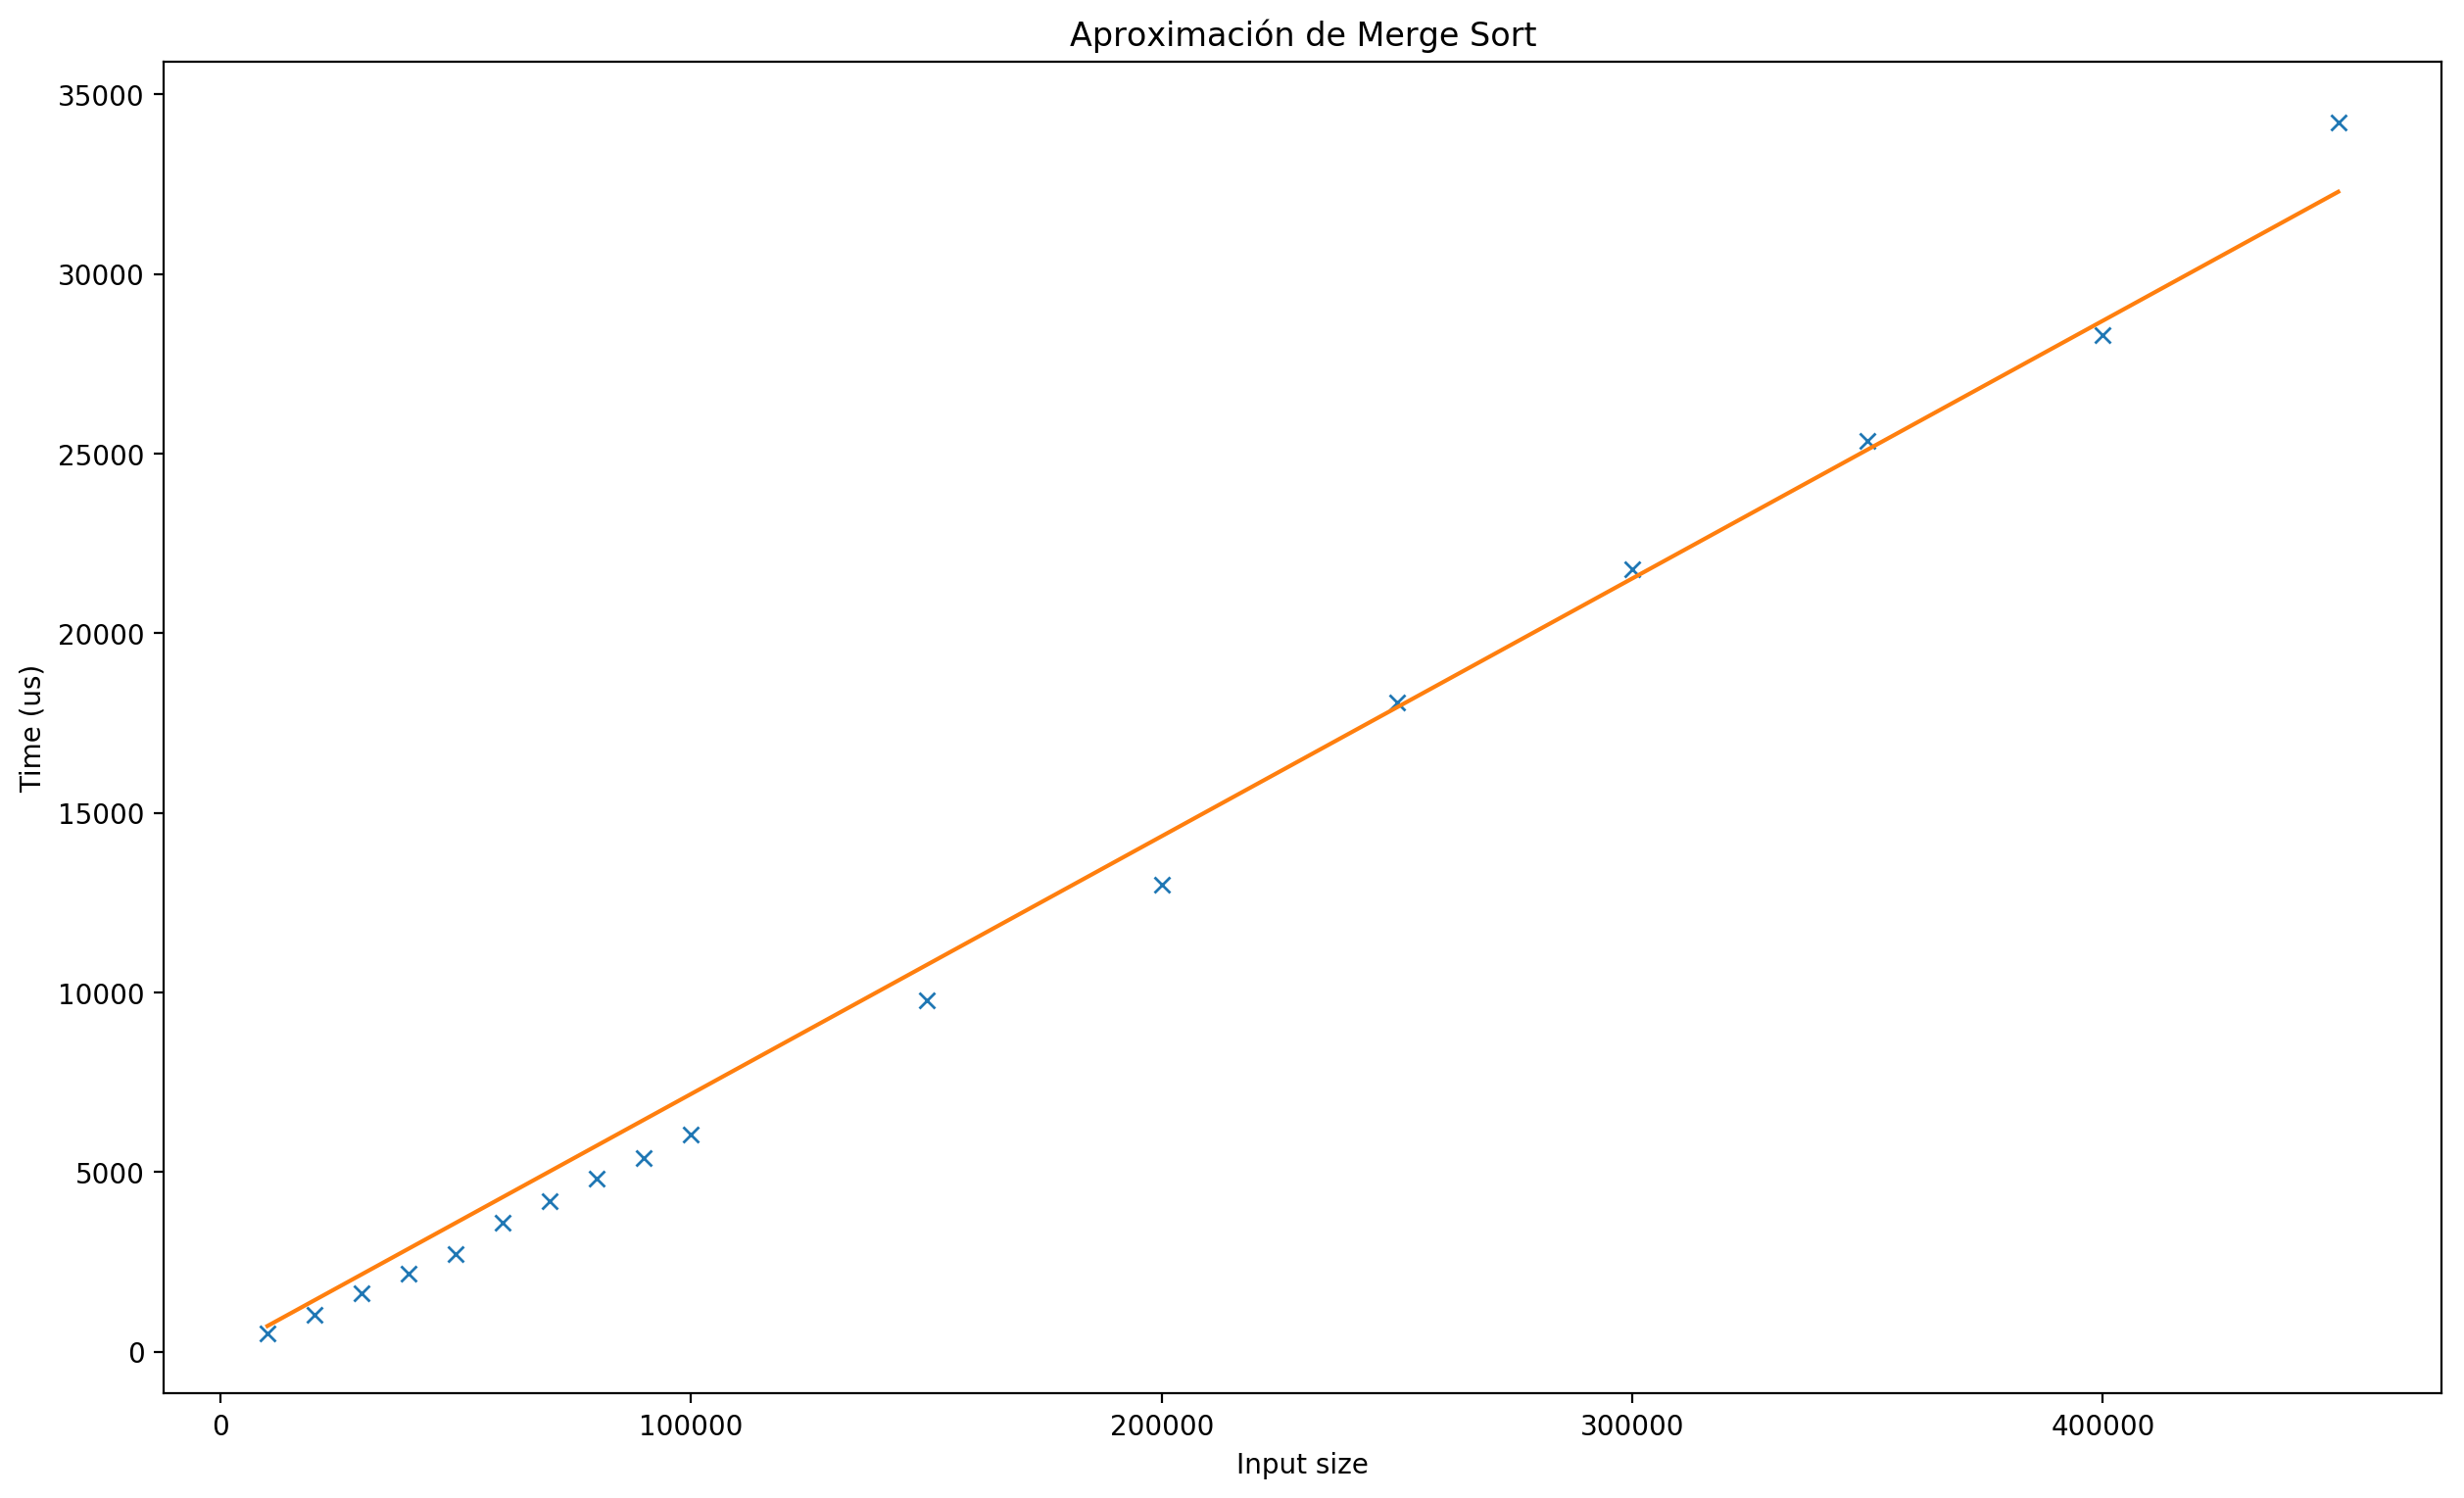
\includegraphics[width=\textwidth]{./Graficas/merge_ajuste.png}
\end{frame}

\begin{frame}[fragile]{Merge Sort. 
	\normalfont{Eficiencia híbrida}}
\textbf{Constante oculta:} $K=1.1670955046281213$

\textbf{Ajuste por regresión:} $T(n)=0.07175341\cdot n\log n$
\begin{itemize}
	\item Error para recta ($kn$): 0.3473246336299704\%
	\item Error para cuadrática ($kn^2$): 14.334551135315282\%
	\item Error para cúbica ($kn^3$): 37.228355082448616\%
	\item Error para logarítmica ($k\log n$): 100.0\%
	\item \textbf{Error para $\boldsymbol{n}$-logarítmica ($\boldsymbol{kn\log n}$): 0.246638483904476\%}
\end{itemize}
\end{frame}

\begin{frame}[fragile]{Hanoi}
\begin{lstlisting}[language=C]
void hanoi(int M, int i, int j) {
	if ( M > 0 ) {
		hanoi(M-1, i, 6-i-j);
		hanoi(M-1, 6-i-j, j);
	}
}
\end{lstlisting}
\end{frame}

\begin{frame}[fragile]{Hanoi. 
\normalfont{Eficiencia teórica}}
Cada iteración el algoritmo se llama a sí mismo dos veces. $$T(n) = 2T(n-1)+1$$ $$(x-2)(x-1) = 0$$ $$T(n) = c_1*2^n+c_2*1^n = c_1*2^n + c_2$$ Por lo que: $$T(n) \in O(2^n)$$
\end{frame}

\begin{frame}[fragile]{Hanoi. 
\normalfont{Eficiencia empírica}}
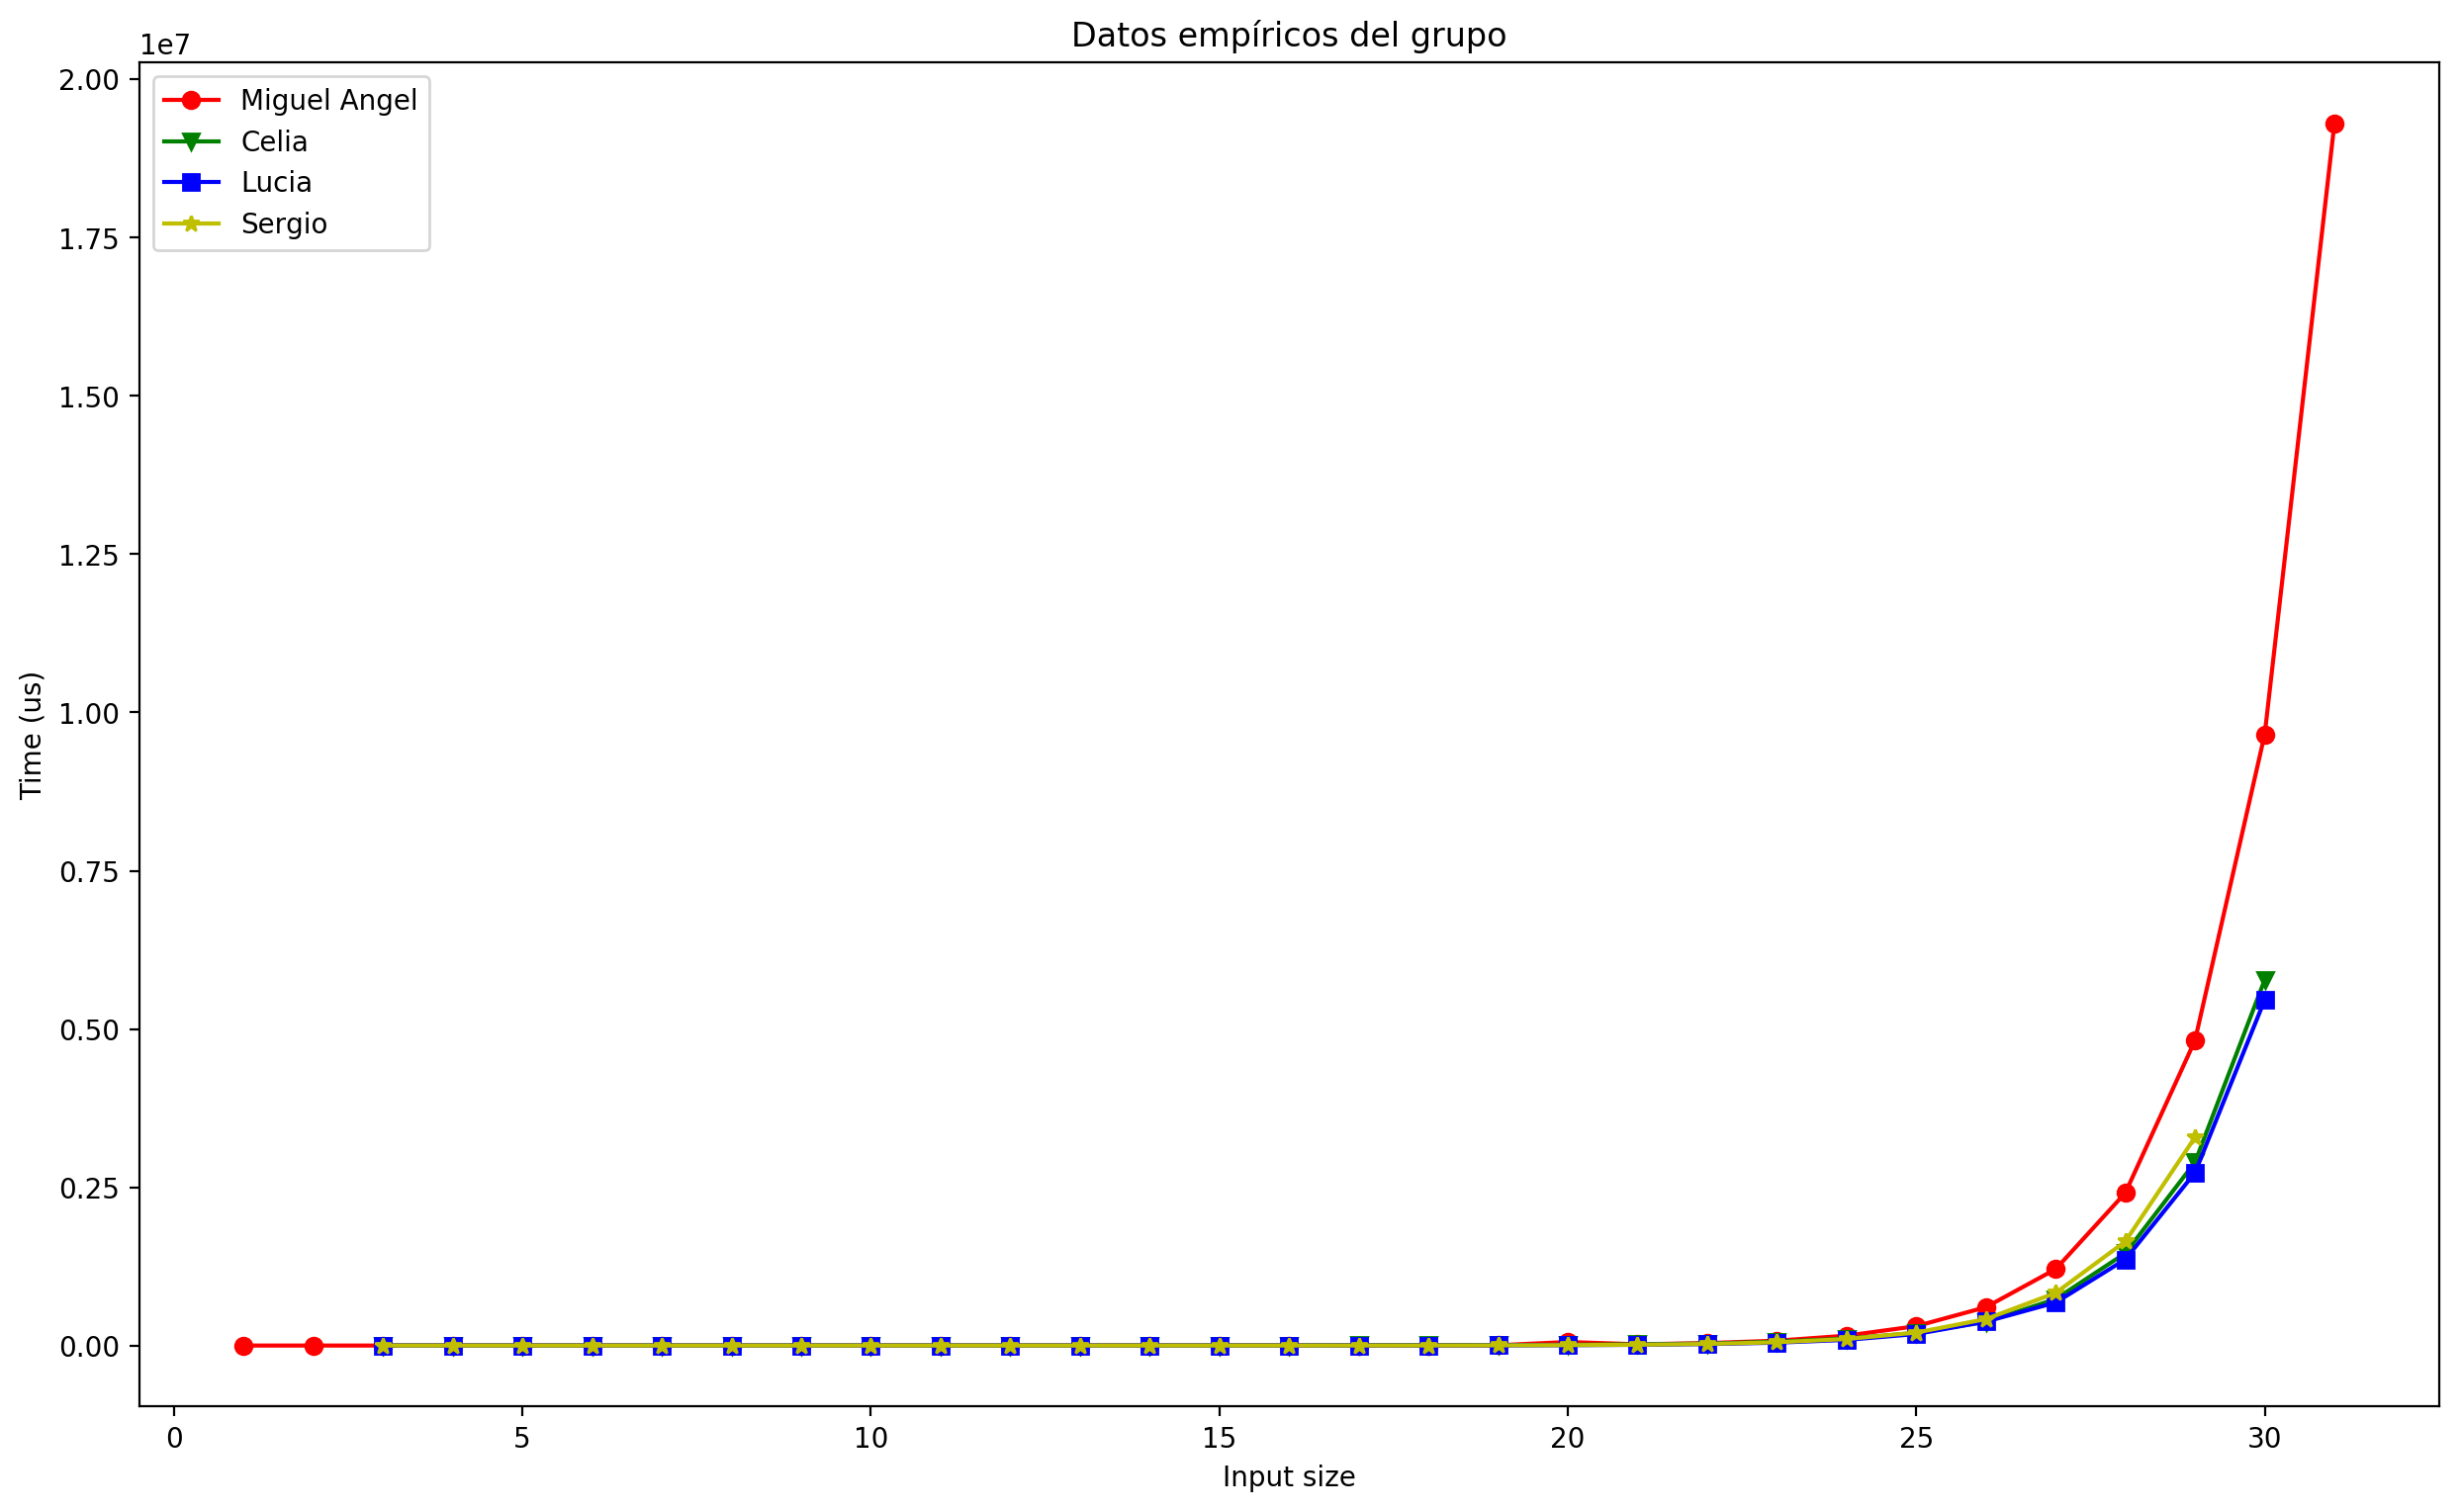
\includegraphics[width=\textwidth]{./Graficas/hanoi_todos.png}
\end{frame}

\begin{frame}[fragile]{Hanoi. 
\normalfont{Eficiencia híbrida}}
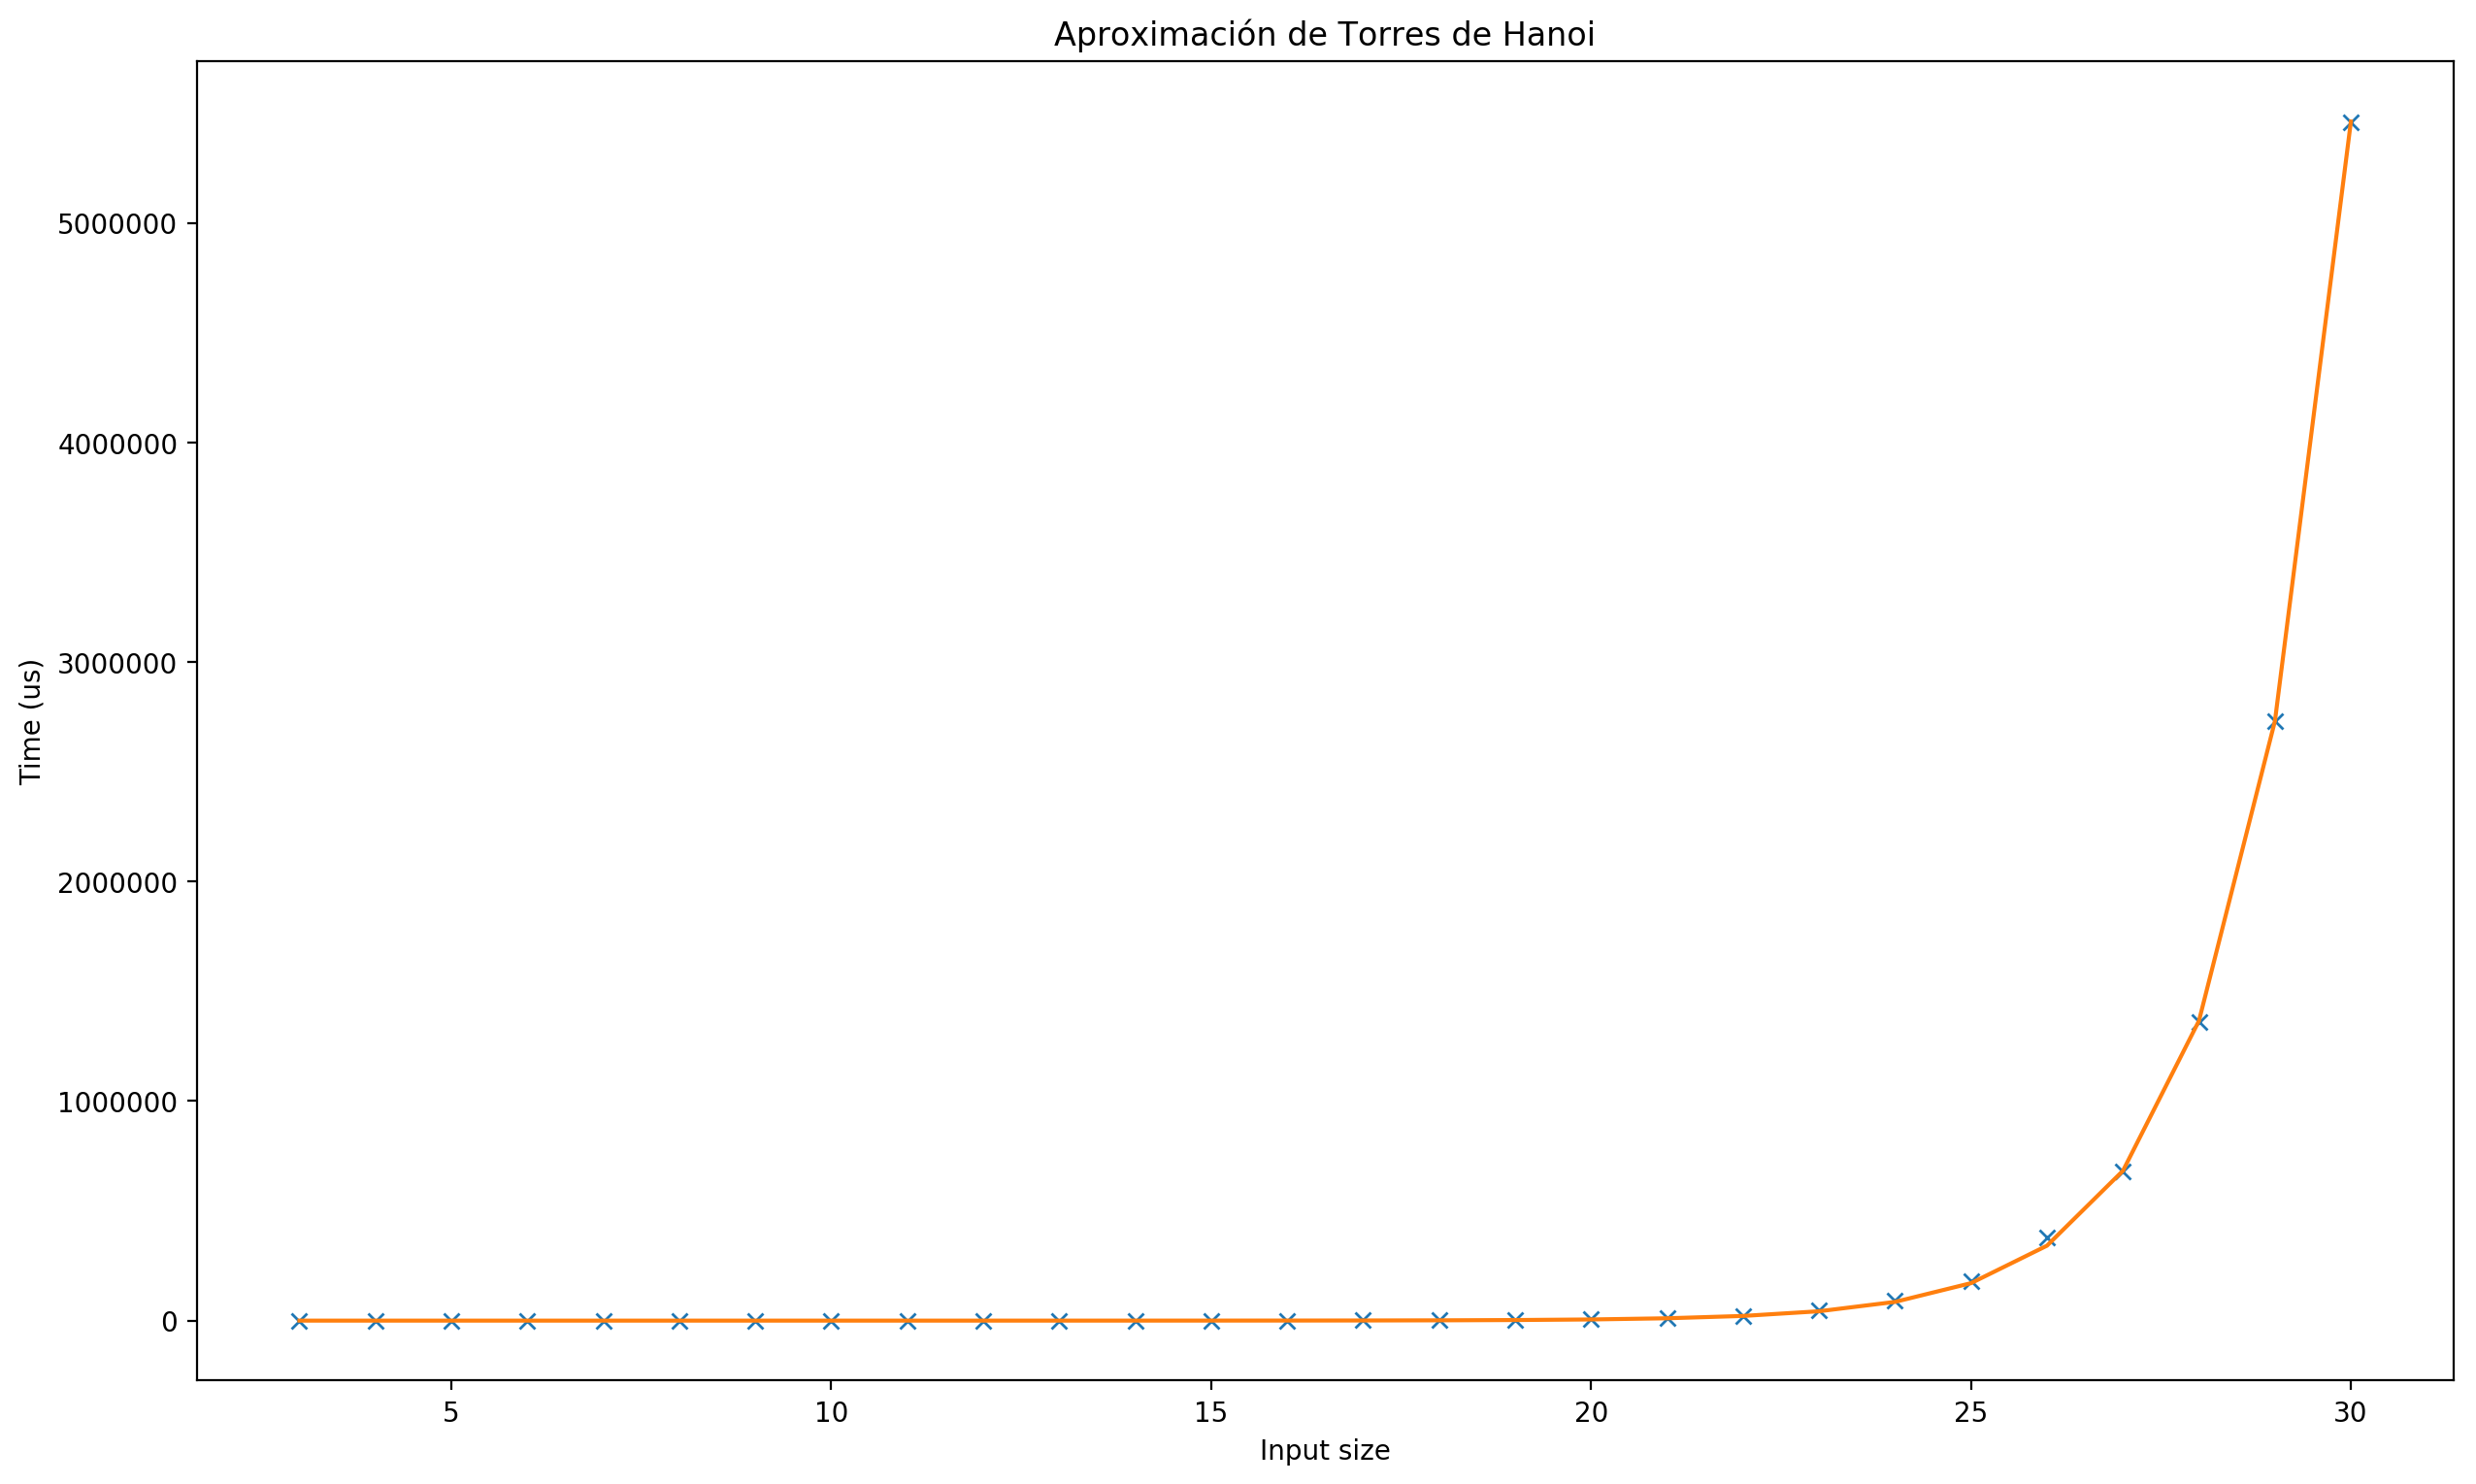
\includegraphics[width=\textwidth]{./Graficas/hanoi_ajuste.png}
\end{frame}

\begin{frame}[fragile]{Hanoi. 
	\normalfont{Eficiencia híbrida}}
\textbf{Constante oculta:} $K=0.7263436302553232$

\textbf{Ajuste por regresión:} $T(n)=0.00508635\cdot 2^n$
\begin{itemize}
	\item Error para recta ($kn$): 76.01343903600339\%
	\item Error para cuadrática ($kn^2$): 71.13401593179258\%
	\item Error para cúbica ($kn^3$): 57.61256154034523\%
	\item Error para exponencial ($ke^n$): 3.1920070654956563\%
	\item \textbf{Error para potencial ($k2^n$): 0.004591299781178793\%}
	\item Error para logarítmica ($k\log n$): 100.0\%
\end{itemize}
\end{frame}

\section{Conclusión}

\begin{frame}{Conclusión}
El análisis teórico ha sido correcto: correcta regresión.

Lo que más influye es la eficiencia del algoritmo.

Dependencia del computador: arquitecturas diferentes y prestaciones diferentes dan lugar a resultados diversos.
\end{frame}


\begin{frame}{Comparativa entre algoritmos de búsqueda}
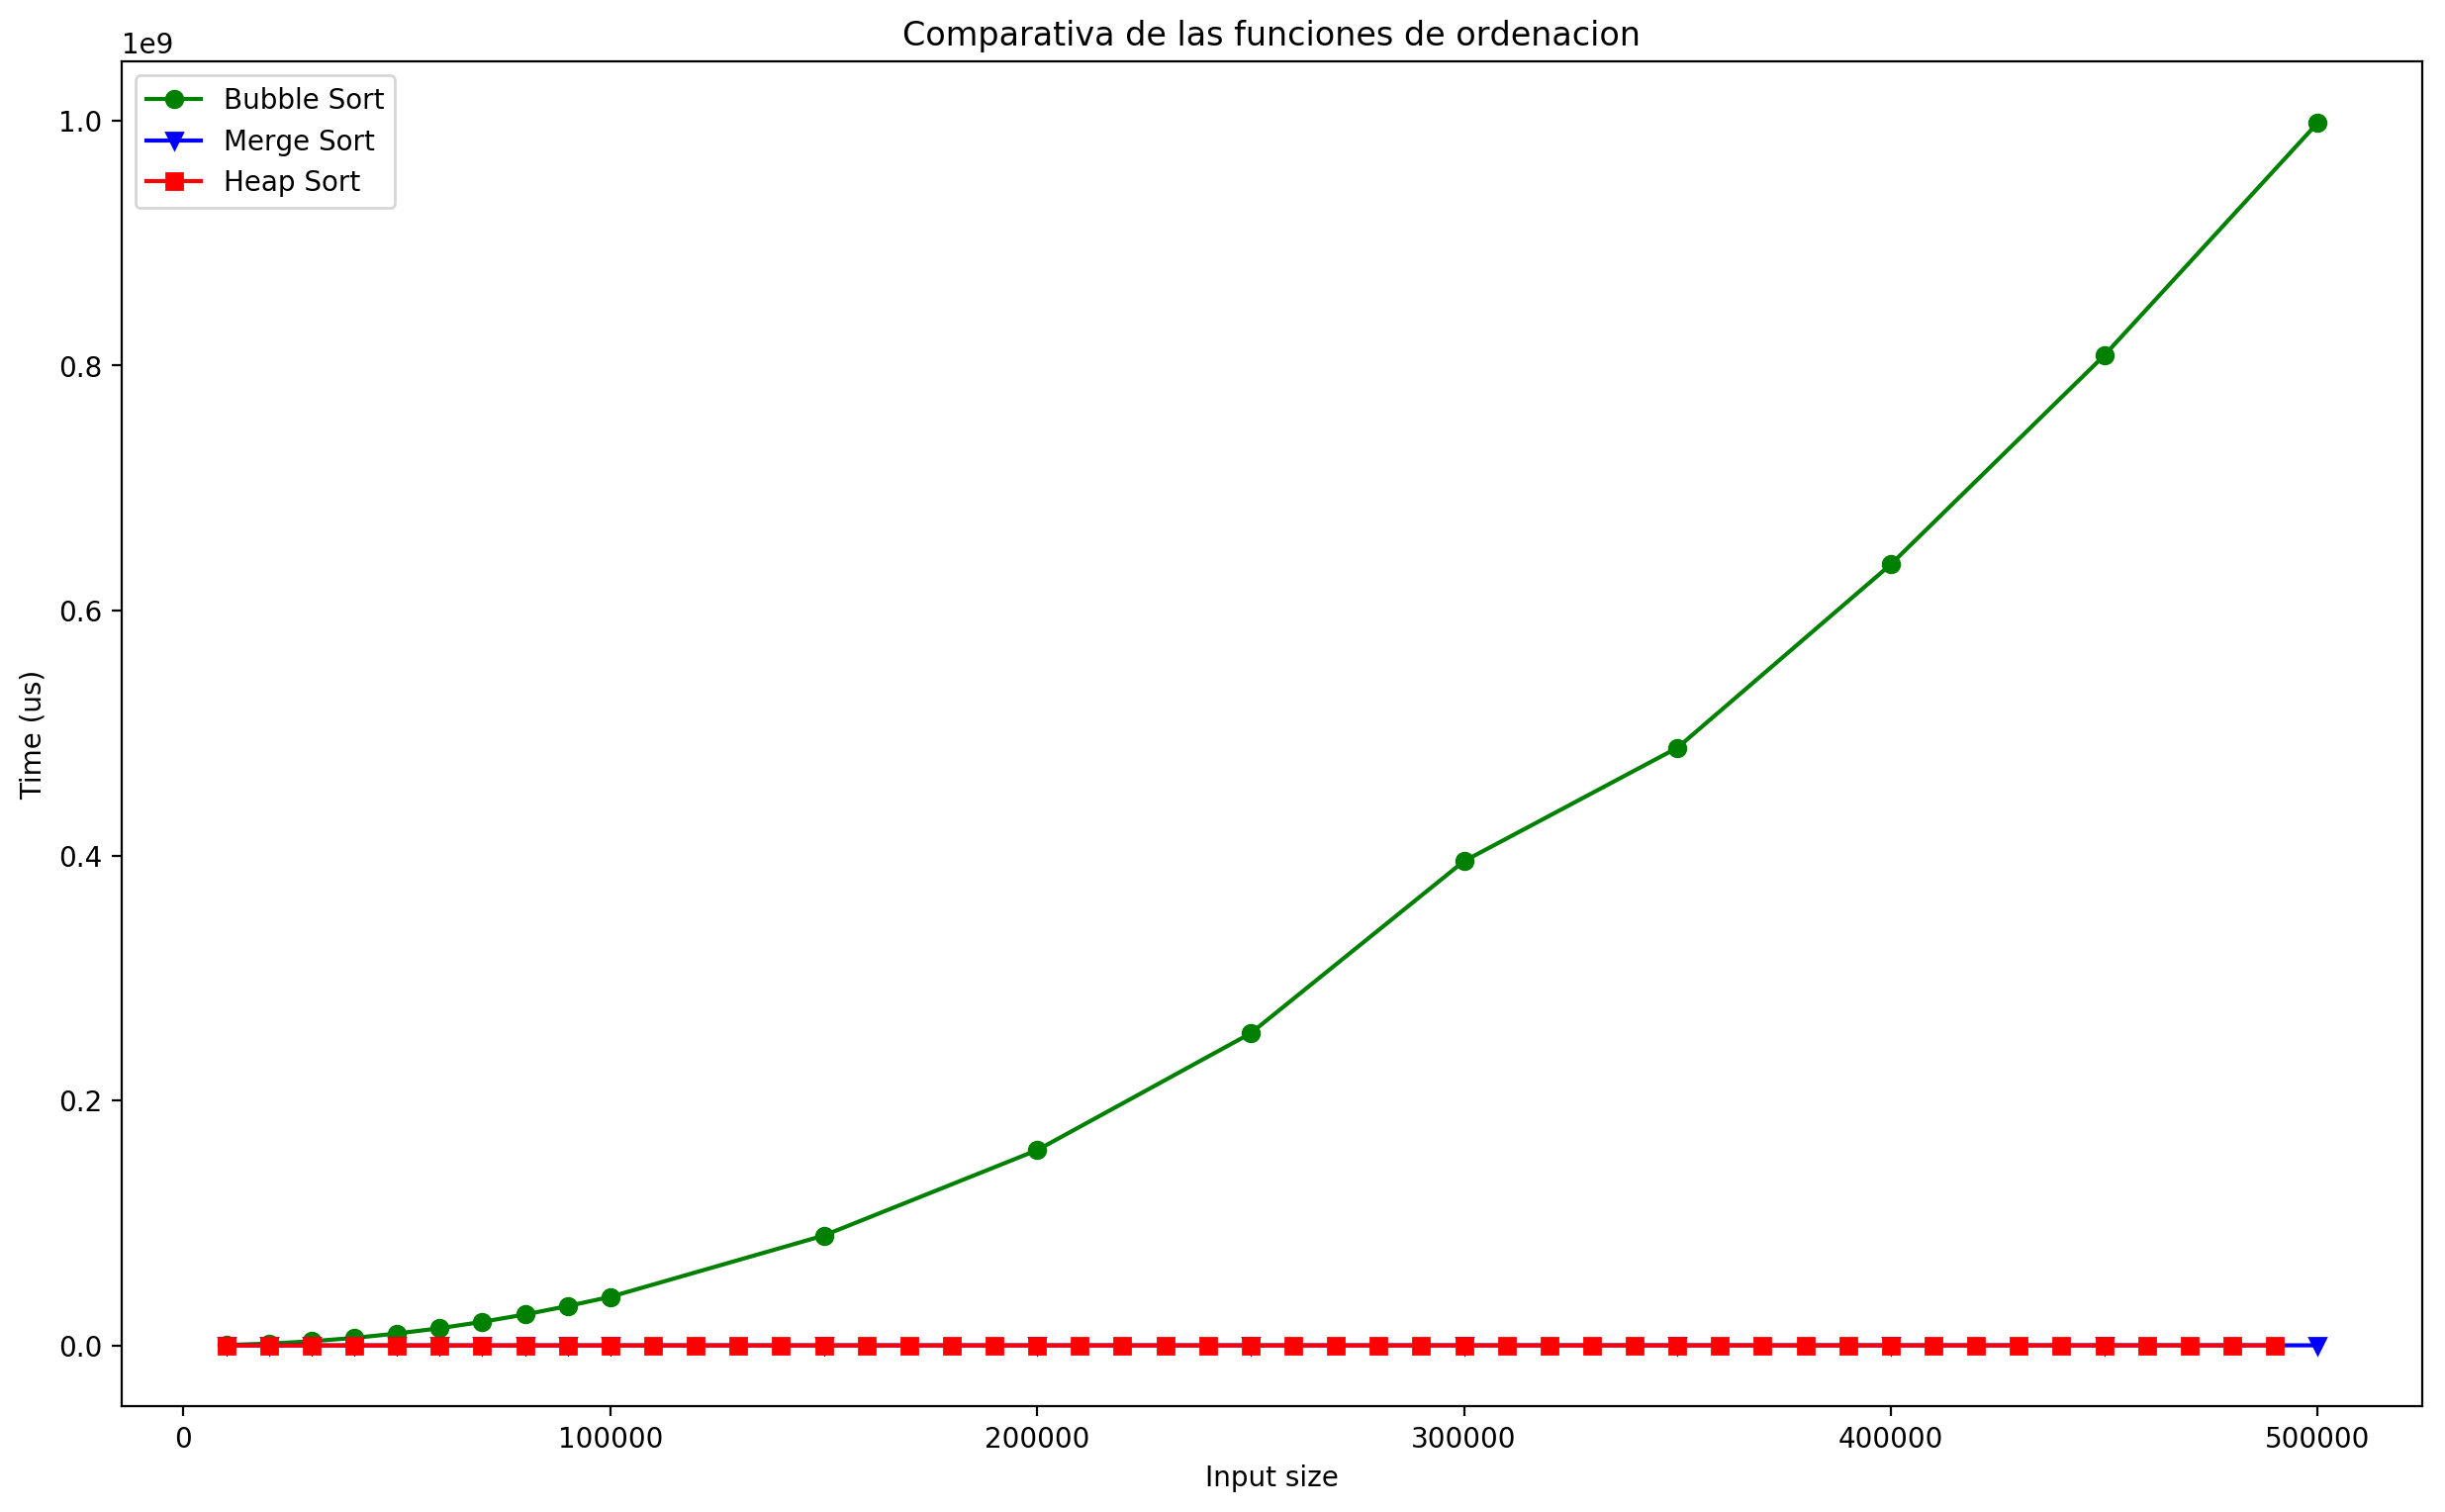
\includegraphics[width=\textwidth]{./Graficas/comparativa_todas.png}
\end{frame}

\begin{frame}{Comparativa entre algoritmos de búsqueda}
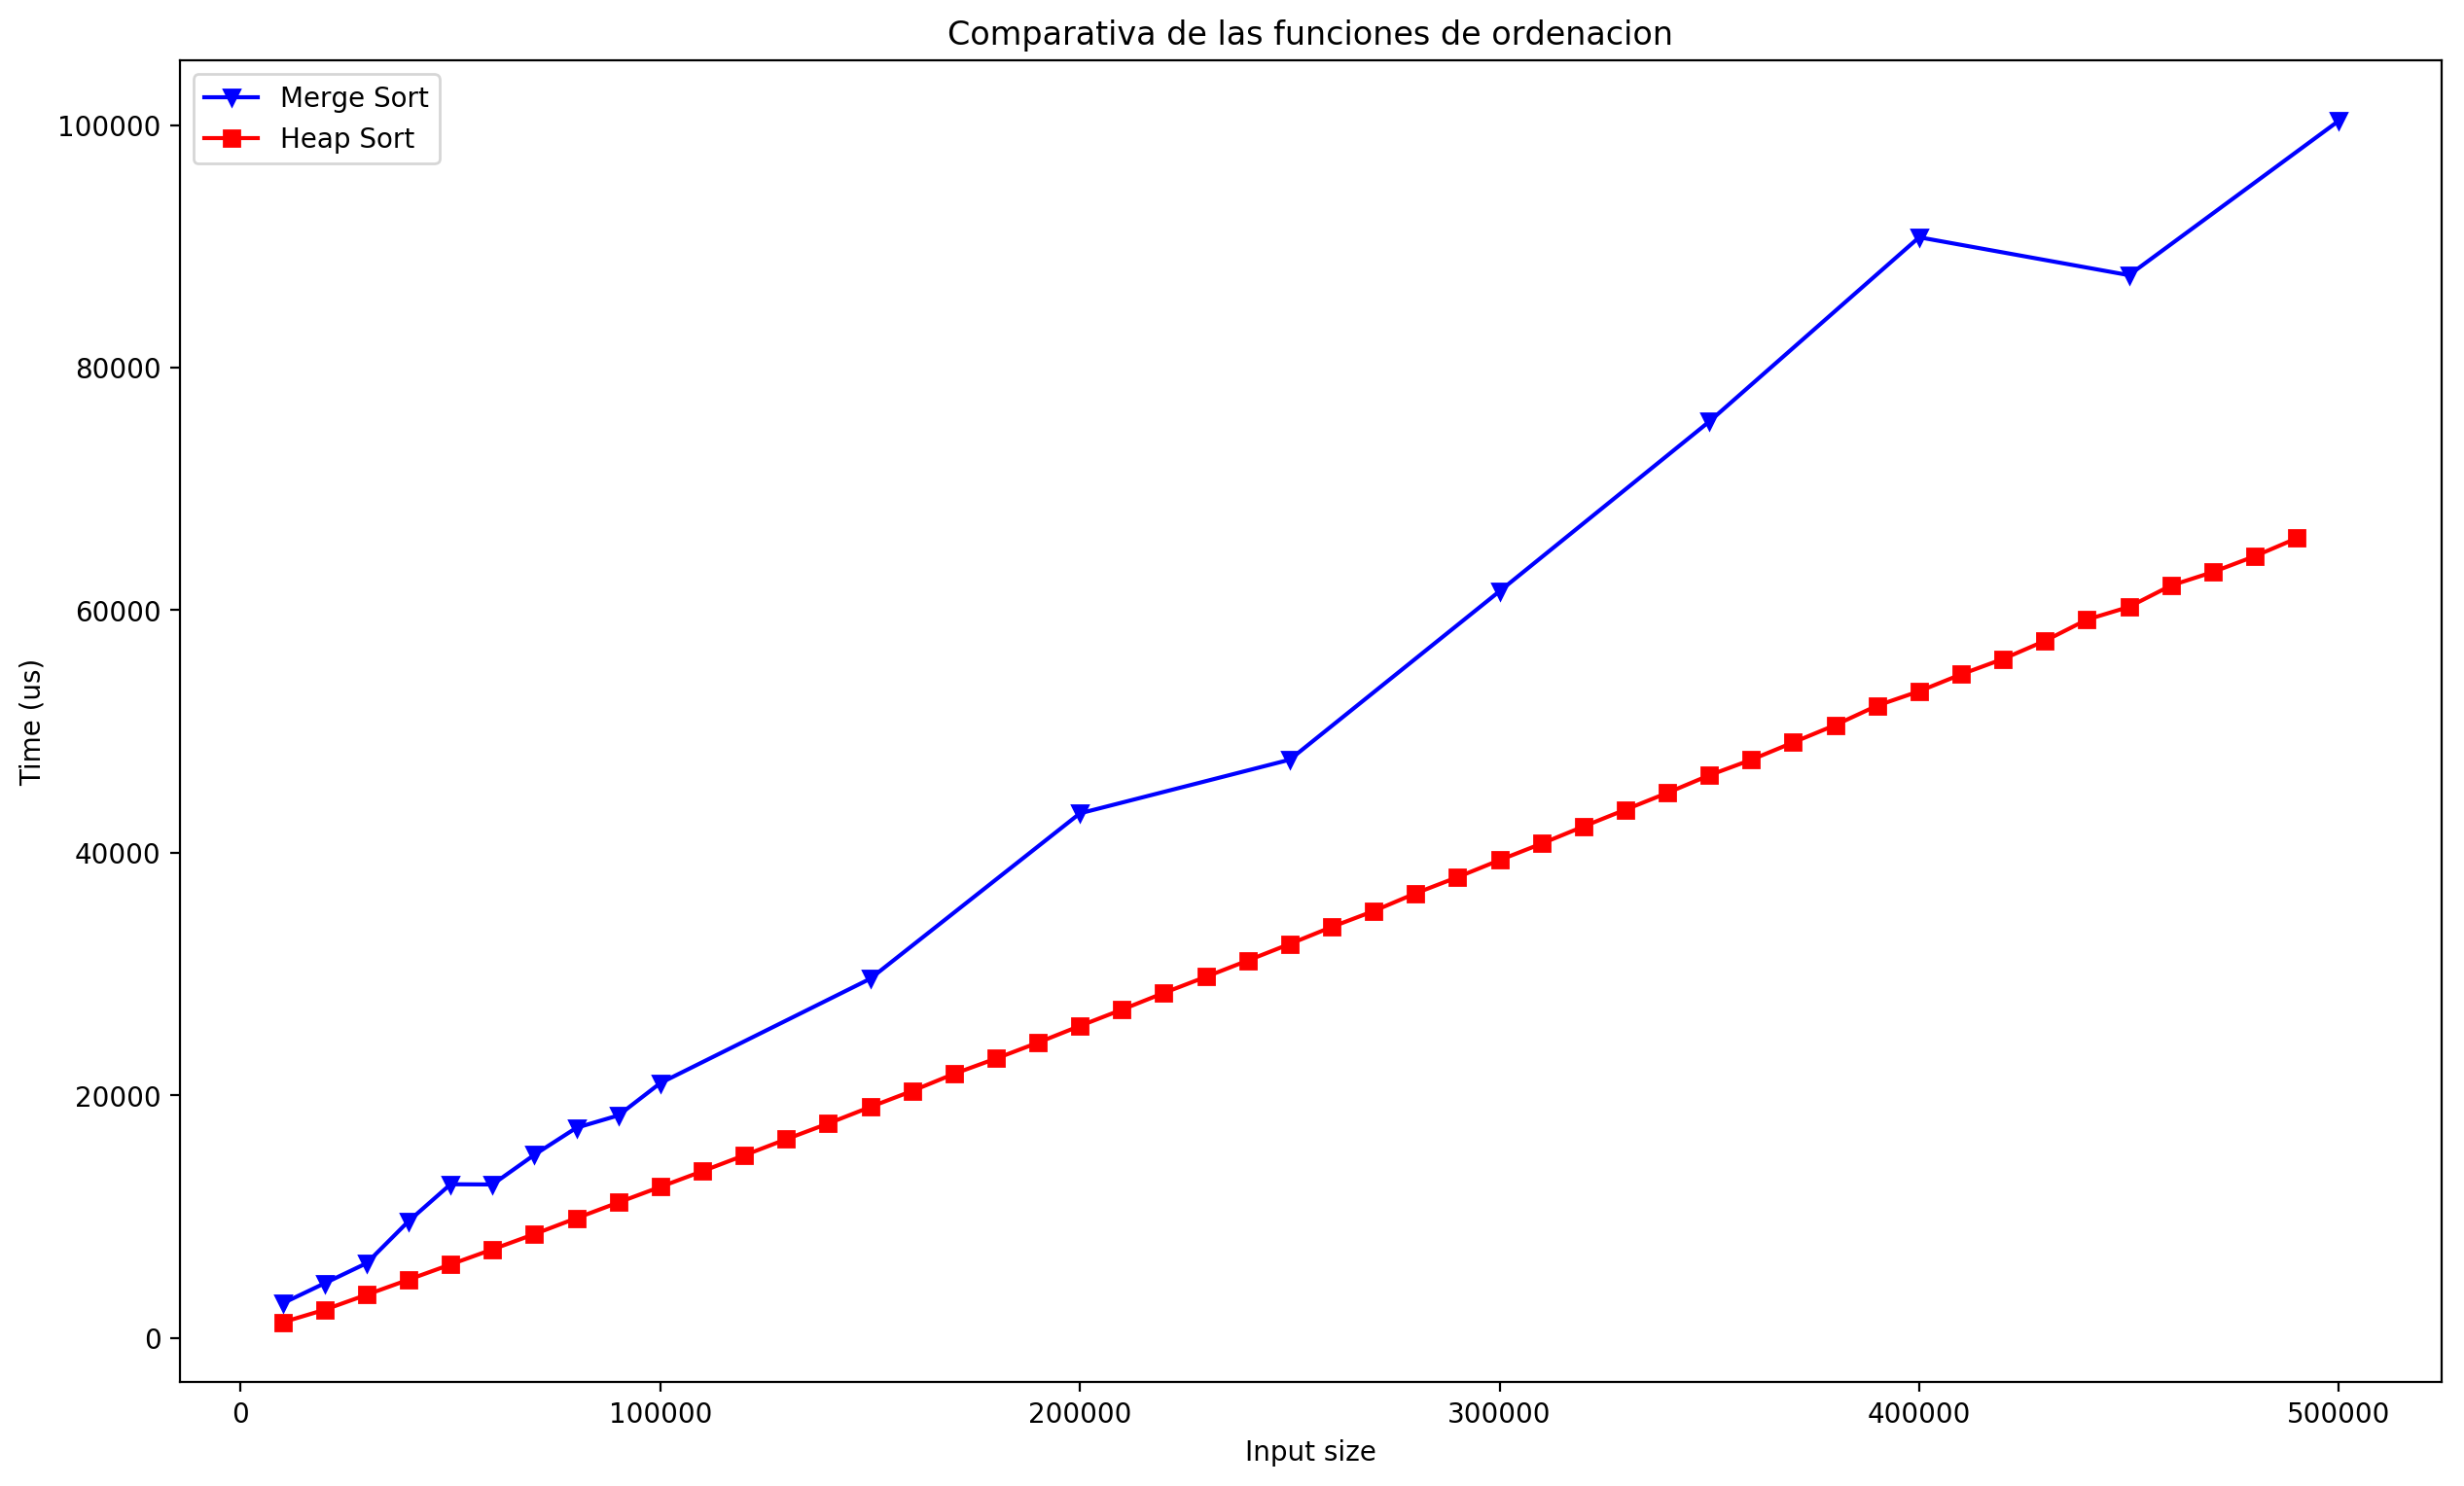
\includegraphics[width=\textwidth]{./Graficas/comparativa_merge_heap.png}
\end{frame}

\end{document}
